\section{Simulación del prototipo}

Las condiciones de simulación y ensayo fueron:

\begin{itemize}
    \item Tensión de entrada: $V_s=36V$
    \item Frecuencia de conmutación: $f=125kHz$
    \item Ciclo de trabajo: $D=0.4$
    \item Resistencia de carga: $R=88.5\Omega$
\end{itemize}

Las formas de onda con color rojo corresponden a las señales medidas mediante el osciloscopio y las de color negro corresponden a las simuladas en LTSpice. 

Previo al análisis se detallan dos problemas encontrados al momento de realizar las mediciones.
En primer lugar, al realizar las mediciones de tensión se evidenció un inconveniente con la tierra de la PCB. 
La fuente regulable de $36V$ eleva notablemente su corriente entregada al circuito 
cuando se conecta la tierra de la punta del osciloscopio en ciertos puntos de la placa. 
Estas mediciones fueron tomadas estableciendo en la fuente un correcto límite de corriente. 
Además, en otros puntos como el transformador de potencia disminuye la tensión entregada por la fuente regulable de $12V$.

En segundo lugar, al utilizar resistencias de $1\Omega$ y potencia nominal $2W$ para medir corrientes en el circuito, 
se detectaron oscilaciones indeseadas en sus formas de onda con una frecuencia de $f_{osc}=1.1MHz$. 
Por lo tanto, se quitaron dichas resistencias y se soldaron cables con un largo tal que se pueda medir 
la corriente a través de los mismos utilizando puntas de corriente para el osciloscopio TEKTRONIX modelo P6021. 
Las mismas están conformadas por un transformador de corriente y, en consecuencia, sólo miden la componente alterna de la señal.
El cable que se introduce es el primario, por lo que consta de una única vuelta, y el secundario está adentro de la punta. 
Pueden variar su sensibilidad seleccionando $2mA/mV$ o $10mA/mV$.
Al medir corriente con las mismas no se detectaron las oscilaciones,
con lo cual se concluye que a la frecuencia de trabajo las resistencias presentan una alta componente inductiva que genera las oscilaciones indeseadas. 
Además, al quitar las resistencias se incrementó levemente la tensión de salida y la eficiencia. 
% % 1) Tensión de salida en el colector del TL494 <<< DONE

% Se verifica que el ciclo de trabajo es de $D=0.4$ y la frecuencia de conmutación es de aproximadamente $f=125kHz$. 
% Su amplitud se reduce considerablemente de los $12V$ que poseía sin la carga del convertidor a $8V$ con el mismo acoplado. 
% La forma de onda presenta una leve deformación respecto a la señal sin carga. 

% % 2) Tensión en el capacitor Ct <<< N/A <<< DONE

% Se observa una disminución en la frecuencia de la forma de onda a aproximadamente $f=112kHz$. 
% El prototipo presenta una oscilación no deseada de $f_{osc}=1.25MHz$, 
% la cual estará presente en muchas de las formas de onda que se analizarán a continuación. 

% % 3) Tensión de salida de la etapa de ganancia de corriente <<< DONE

% Dado que la etapa posee ganancia de tensión unitaria, su forma de onda es aproximadamente igual a la tensión de salida del TL494. 
% Las oscilaciones fueron eliminadas mediante la red snubber. 

% % 4) Tensión en el primario del transformador del driver <<< DONE

% La amplitud y la forma de onda de la señal del prototipo coinciden respecto a la simulación. 
% Se observan unos picos en los flancos de subida y de bajada. 

% % 5) Tensión en el secundario del transformador del driver <<< DONE

% La amplitud y la forma de onda de la señal del prototipo coinciden respecto a la simulación. 
% Se observa un pico en el flanco de bajada. 

% % 6) Corriente en el primario del transformador del driver <<< DONE

% La forma de onda del prototipo está deformada y posee levemente mayor amplitud. 

% % 7) Corriente en la resistencia entre gate y source del driver <<< DONE

% La amplitud y la forma de onda de la señal del prototipo coinciden respecto a la simulación. 
% Presenta la oscilación de $f_{osc}=1.25MHz$. 

% % 8) Corriente que circula por el gate del MOSFET 1 (high side) <<< DONE

% El prototipo presenta una segunda onda triangular negativa indeseada. 
% Además, sus picos de amplitud son mayores. 

% % 9) Corriente que circula por el gate del MOSFET 2 (low side) <<< DONE

% El prototipo presenta un pico negativo indeseado. 
% Presenta la oscilación de $f_{osc}=1.25MHz$. 

% % 10) Corriente que circula por el drain del MOSFET 1 (high side) <<< DONE

% La amplitud del prototipo es 1A menor respecto a la simulada debido a que las puntas de corriente desacoplan la continua. 

% % 11) Corriente que circula por el drain del MOSFET 2 (low side) <<< DONE

% La amplitud del prototipo es 1A menor respecto a la simulada debido a que las puntas de corriente desacoplan la continua. 

% % 12) Corriente en el primario del transformador de potencia  <<< DONE

% La amplitud del prototipo es menor respecto a la simulada debido a que las puntas de corriente desacoplan la continua. 

% % 13) Corriente en el inductor del filtro de salida <<< DONE

% La amplitud de la forma de onda del prototipo es 30mA menor a la simulada. 
% Además, presenta una oscilación de $f=3.68MHz$ en la rampa de subida y de $f=38.5MHz$ en la de bajada. 

% % 14) Corriente por la carga y su ripple <<< DONE
% % Revisar valor

% Su amplitud es 30mA menor a la simulada y presenta una oscilación de $f=34MHz$.

% % 15) Tensión entre gate y source del MOSFET 1 (high side) <<< DONE

% La amplitud y la forma de onda de la señal del prototipo coinciden respecto a la simulación.
% Presenta la oscilación de $f_{osc}=1.25MHz$. 

% % 16) Tensión entre drain y source del MOSFET 1 (high side) <<< DONE

% Exceptuando el pico, la amplitud y la forma de onda de la señal del prototipo coinciden respecto a la simulación.
% Presenta la oscilación de $f_{osc}=1.25MHz$. 

% % 17) Tensión entre gate y source del MOSFET 2 (low side) <<< DONE
% % REPETIDA

% Es la tensión de salida de la etapa de ganancia de corriente.

% % 18) Tensión entre drain y source del MOSFET 2 (low side) <<< DONE

% Exceptuando el pico, la amplitud y la forma de onda de la señal del prototipo coinciden respecto a la simulación.
% Presenta la oscilación de $f_{osc}=1.25MHz$. 

% % 19) Tensión en el primario del transformador de potencia  <<< DONE

% La forma de onda del prototipo difiere de la simulada. 
% Tiene un pico en el flanco de bajada. 
% Presenta la oscilación de $f_{osc}=1.25MHz$. 

% % 20) Tensión en el secundario del transformador de potencia  <<< DONE
% % ADJUNTAR AMBAS IMÁGENES 

% Con una relación 1:1, la tensión en el secundario era de 44V, mucho menor a la tensión en el primario. 
% Con una relación 1:2, la tensión en el secundario es de 68V, aproximadamente igual a la del primario.
% Presenta oscilaciones de $f_{osc_{1}}=3.23MHz$ en la subida y en la bajada y de $f_{osc_{2}}=2.63MHz$ anterior a la subida. 

% % 21) Tensión de salida sobre la carga y su ripple  <<< DONE

% El ripple del prototipo es de 80mV fino y 200mV grueso. Dio peor la captura
% Luego de 120mV. Presenta una oscilación de 2MHz. 

% % 22) Tensión en el inductor del filtro de salida <<< Da como el culo

% El prototipo presenta una oscilación de $f_{osc}=3.03MHz$. 

% % 23) Corriente de salida por colector del TL494 
% % 24) Tensión cátodo ánodo en el diodo D1
% % 25) Tensión cátodo ánodo en el diodo D2
% % 26) Tensión cátodo ánodo en el diodo D3

% El prototipo presenta una oscilación de $f_{osc}=3.03MHz$. 

% % 27) Tensión cátodo ánodo en el diodo D4

% El prototipo presenta una oscilación de $f_{osc}=3.03MHz$. 

% % 28) Corriente en el secundario del transformador de potencia

% El prototipo presenta una oscilación de $f_{osc}=5.26MHz$.

\subsection{Generador de señal PWM}

No se realizarán comparaciones ya que su circuito no fue simulado debido a la ausencia de un correcto modelo del TL494.
El mismo fue probado en una protoboard y luego incluido en el circuito impreso.
En las figuras \ref{fig:osc_pwm_vout_no_snubber} y \ref{fig:osc_pwm_vout_disconnected} se observa la tensión a la salida del TL494 sin la red snubber y con su inclusión respectivamente.
% Sus formas de onda más importantes se compararán con las indicadas en la hoja de datos del fabricante.
\begin{figure}[H]
    \centering
    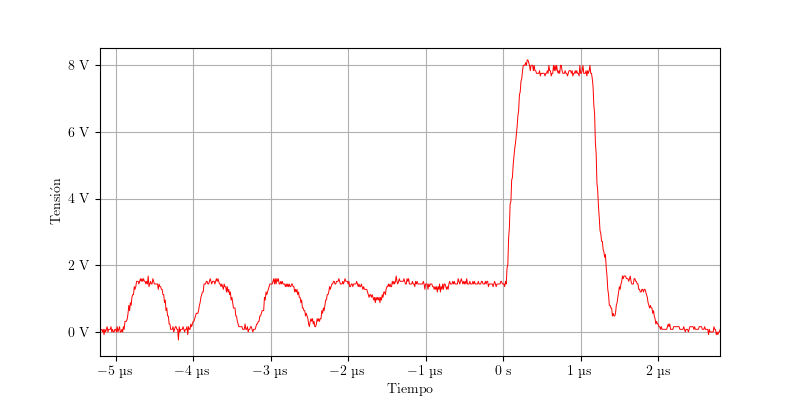
\includegraphics[width=0.8\textwidth]{images/capturas-osciloscopio/TL494/pwm_vout_connected.png}
    \caption{Tensión a la salida del TL494 previo a la implementación de la red snubber}
    \label{fig:osc_pwm_vout_no_snubber}
\end{figure}

\begin{figure}[H]
    \centering
    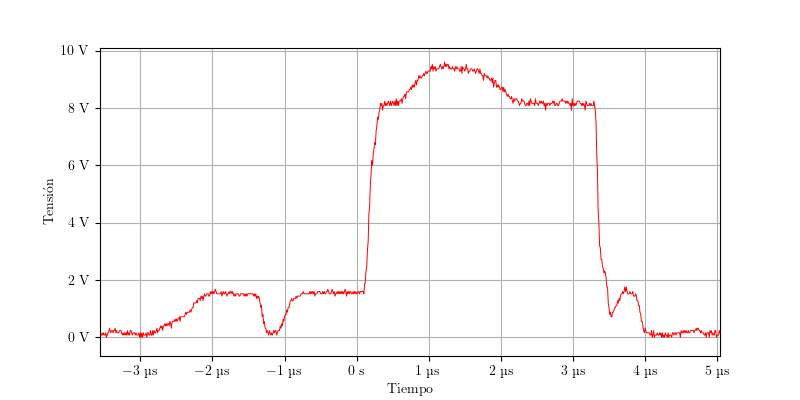
\includegraphics[width=0.8\textwidth]{images/capturas-osciloscopio/17-11-2022/1.png}
    \caption{Tensión a la salida del TL494}
    \label{fig:osc_pwm_vout_disconnected}
\end{figure}

% Se verifica que el ciclo de trabajo es de $D=0.4$ y la frecuencia de conmutación es de aproximadamente $f=125kHz$. 
% Su amplitud se reduce considerablemente de los $12V$ que poseía sin la carga del convertidor a $8V$ con el mismo acoplado. 
% La forma de onda presenta una leve deformación respecto a la señal sin carga. <<< Comparando con otras formas de onda, esta está casi identica
Se puede observar como la red snubber logra eliminar casi por completo la oscilación de alta frecuencia. 
La señal obtenida posee un período $8\mu s$ y se mantiene encendida durante $3.2\mu s$, verificando la frecuencia de conmutación elegida de ($f=125kHz$) y un ancho de pulso ($D=0.4$).
Respecto a la señal sin el convertidor conectado, la forma de onda se distorsiona y su amplitud disminuye de $12V$ a $8V$.
En la figura \ref{fig:sim:osc_pwm_vout} se muestra la misma forma de onda simulada en LTspice.

\begin{figure}[H]
    \centering
    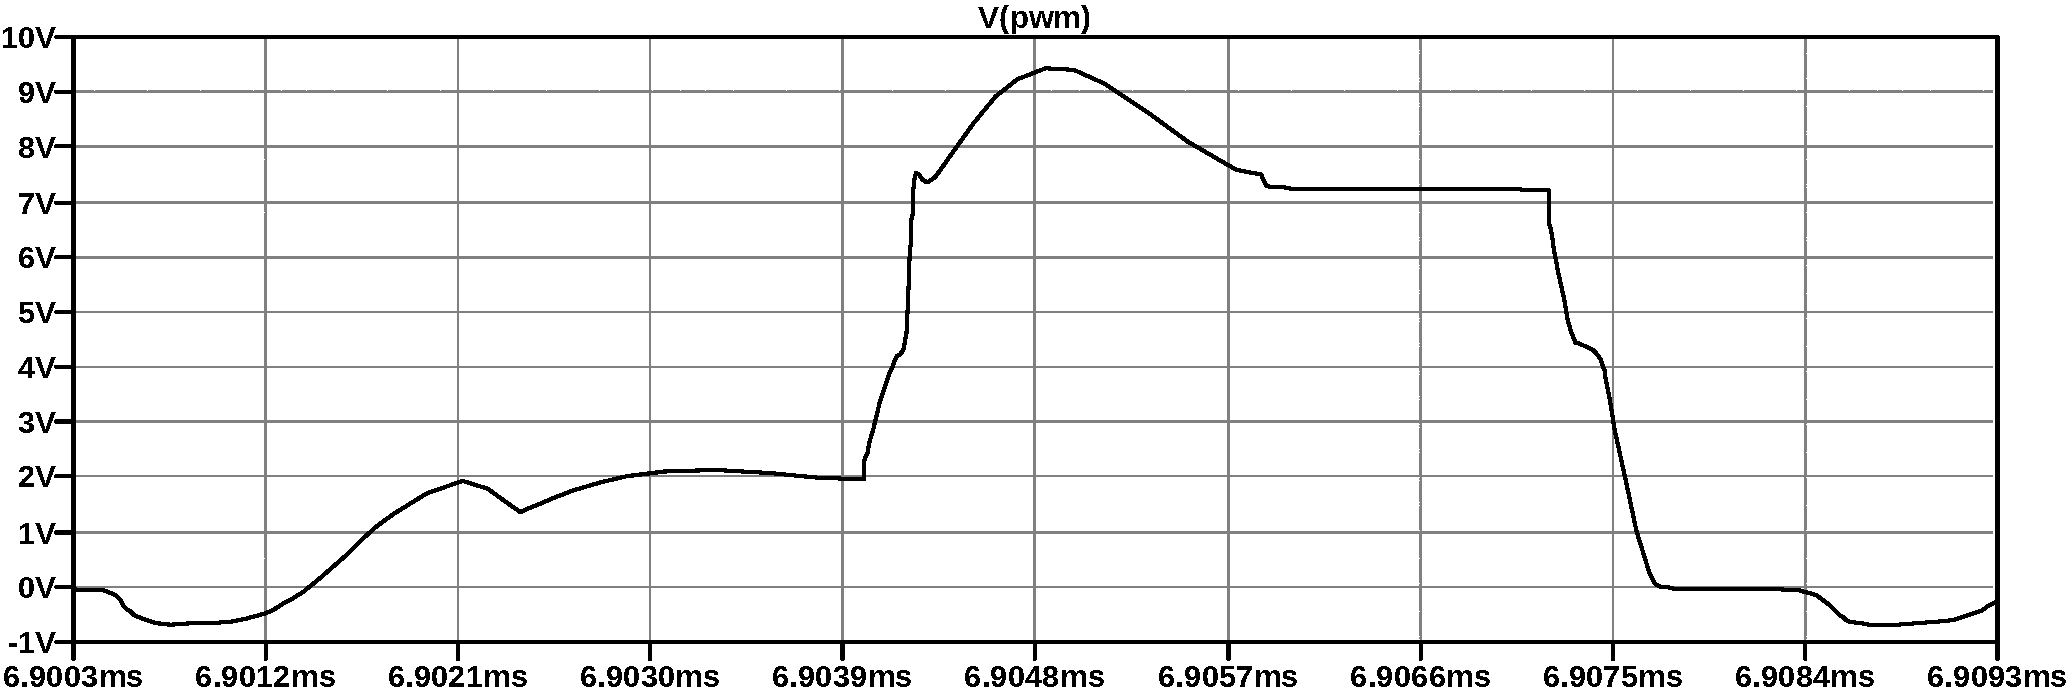
\includegraphics[width=\textwidth]{images/sim/3.pdf}
    \caption{Simulación de la tensión a la salida del TL494}
    \label{fig:sim:osc_pwm_vout}
\end{figure}

En la figura \ref{fig:ct_v} se muestran la tensión en el capacitor $C_t$.
La frecuencia de la forma de onda disminuye a aproximadamente $f=112kHz$ y se percibe la oscilación no deseada de $f_{osc}=1.25MHz$, 
la cual fue eliminada de la señal PWM que excita al MOSFET de lado bajo mediante la red snubber, pero estará presente en muchas de las formas de onda que se analizarán a continuación. 

\begin{figure}[H]
    \centering
    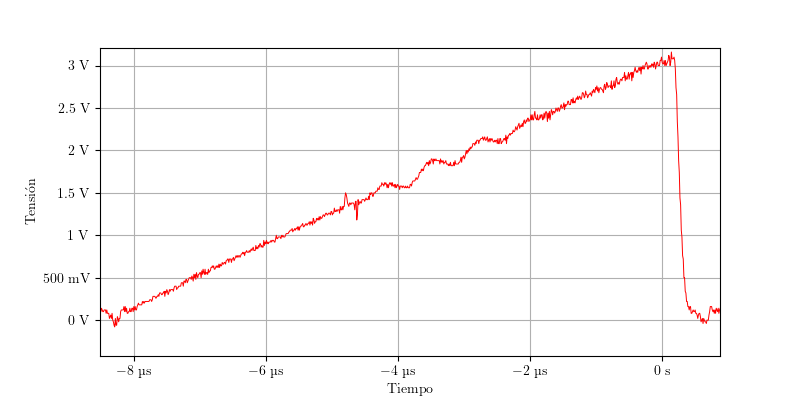
\includegraphics[width=\textwidth]{images/capturas-osciloscopio/17-11-2022/5.png}
    \caption{Tensión en el capacitor $C_t$} %COMPLETAR
    \label{fig:ct_v}
\end{figure}

% 1) Señal PWM

% Se toma la salida por el colector de los transistores del circuito integrado. 
% Su forma de onda son pulsos rectangulares. 
% Amplitud: 0V a Vdrv dados por la tensión de alimentación.
% Frecuencia de 125kHz dada por el capacitor Ct=1nF y $Rt=8k\Omega$ mediante el potenciómetro. 
% Tiempo de encendido: permite controlar el ciclo de trabajo mediante un potenciómetro. 
% Esta señal se mide en 3 condiciones diferentes: 
% A) Sin el convertidor forward conectado
% B) Con el convertidor forward conectado pero sin su alimentación de 36V
% C) Con el convertidor forward conectado y alimentado

% 2) Diente de Sierra 

% Tensión en el capacitor Ct. 

% 3) Tensión en el puerto DTC 

\subsection{Etapa de ganancia de corriente}

% En las figuras \ref{fig:pwm_iout_sin_bjt} y \ref{fig:pwm_iout_con_bjt} puede observarse la corriente de salida del TL494 antes y después de agregar la etapa de ganancia de corriente, respectivamente.

% \begin{figure}[H]
%     \centering
%     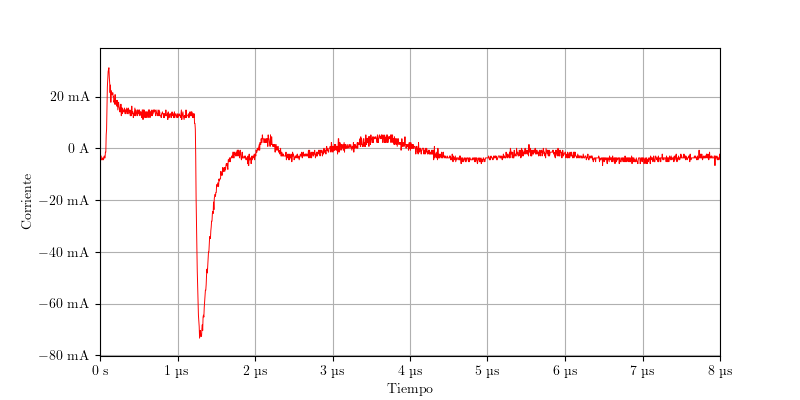
\includegraphics[width=\textwidth]{images/capturas-osciloscopio/TL494/pwm_iout_sin_bjt.png}
%     \caption{Corriente a la salida del TL494 sin colocar la etapa intermedia de ganancia de corriente}
%     \label{fig:pwm_iout_sin_bjt}
% \end{figure}

% \begin{figure}[H]
%     \centering
%     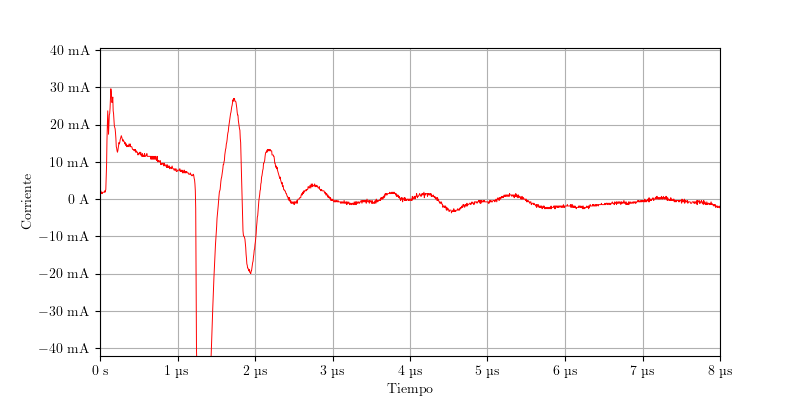
\includegraphics[width=\textwidth]{images/capturas-osciloscopio/BJT/bjt-iin-con-etapa.png}
%     \caption{Corriente a la salida del TL494 con la etapa intermedia de ganancia de corriente}
%     \label{fig:pwm_iout_con_bjt}
% \end{figure}

% Puede observarse que las oscilaciones aumentan. %WHAT?
Dado que la carga que genera el convertidor sobre el TL494 es muy alta, sin una etapa de ganancia de corriente, la forma de onda PWM 
se distorsionaba y disminuía notablemente su amplitud, lo que causaba que los MOSFETs no se saturaran y aumentaran demasiado su temperatura.
Los resultados obtenidos con la inclusión de esta etapa fueron una mejora en la forma de onda de la señal PWM y un incremento notorio en su amplitud.
Sin embargo, actualmente su amplitud disminuye al aumentar el ciclo de trabajo.

En la figura \ref{fig:osc:3} se muestra la tensión de salida de la etapa de ganancia de corriente.
Al igual que la tensión a la salida del TL494, esta señal PWM que controla al MOSFET de lado bajo verifica las condiciones de funcionamiento con un período de $8\mu s$ y un ancho de pulso de aproximadamente 40\%.
Además se observa un mejor resultado en la forma de onda respecto a la simulación de la figura \ref{fig:sim:3}. %Porque estamos re masa.

% Dado que la etapa posee ganancia de tensión unitaria, su forma de onda es aproximadamente igual a la tensión de salida del TL494. 
% Las oscilaciones fueron eliminadas mediante la red snubber. 

\begin{figure}[H]
    \centering
    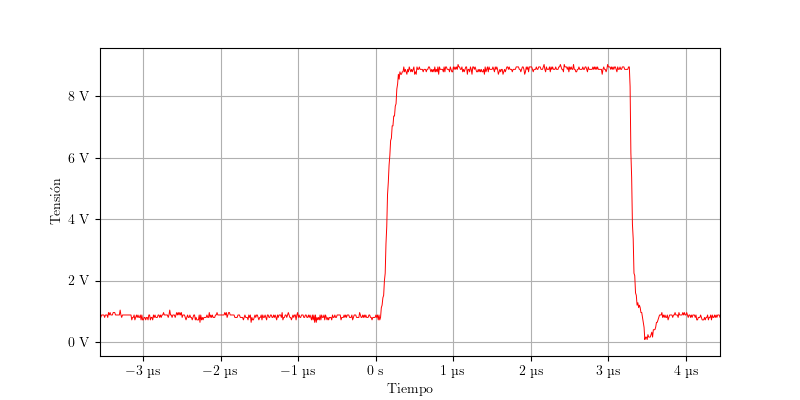
\includegraphics[width=0.8\textwidth]{images/capturas-osciloscopio/17-11-2022/3.png}
    \caption{Tensión a la salida de la etapa de ganancia de corriente}
    \label{fig:osc:3}
\end{figure}

\begin{figure}[H]
    \centering
    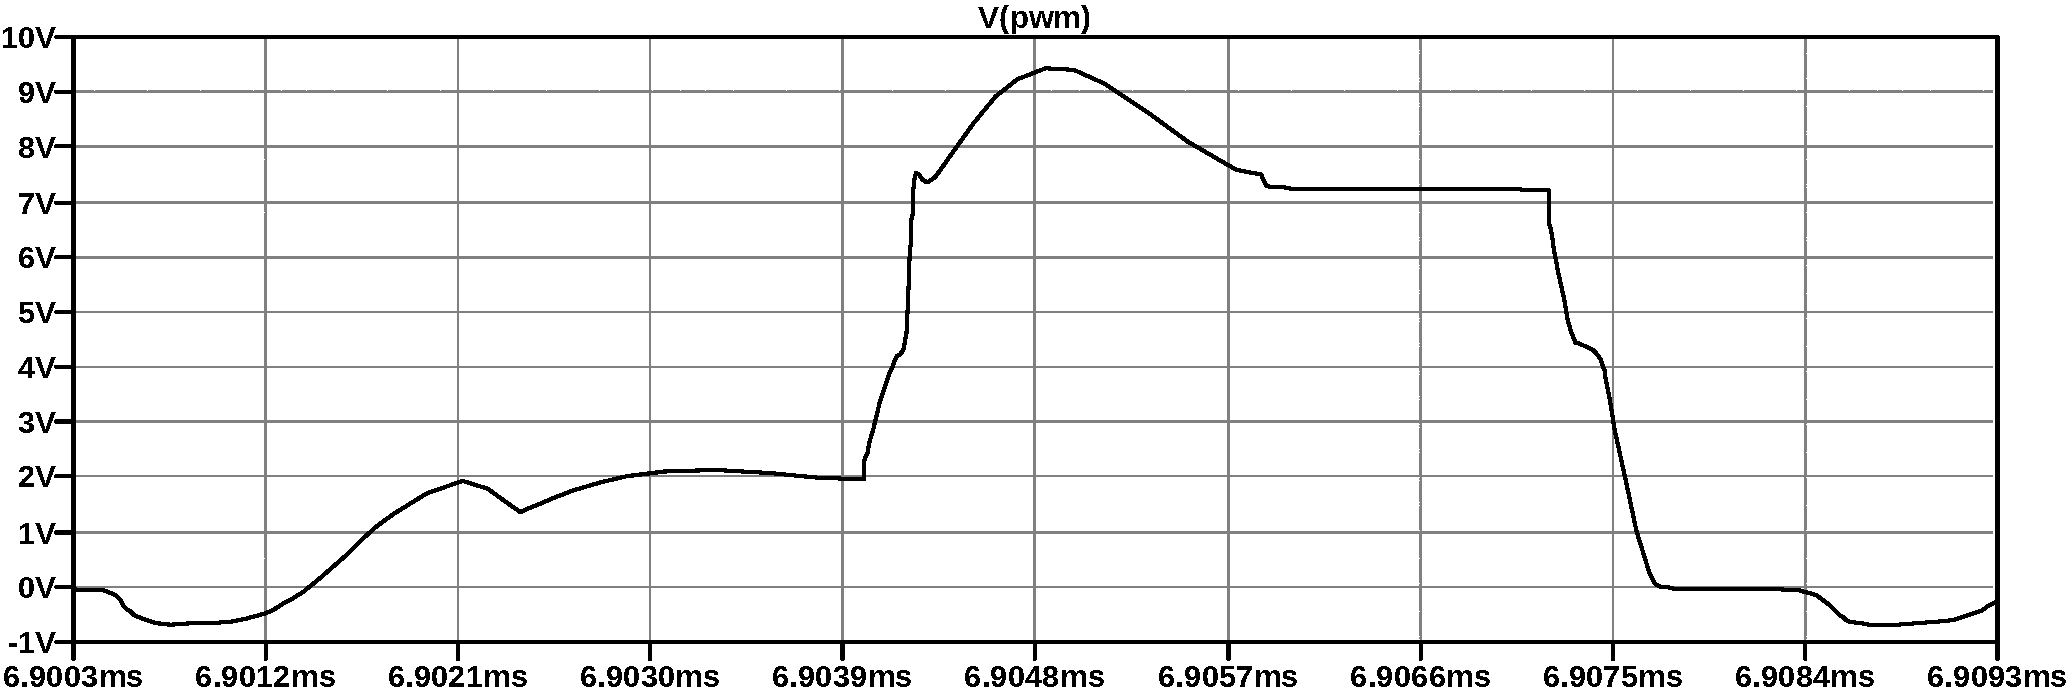
\includegraphics[width=\textwidth]{images/sim/3.pdf}
    \caption{Simulación de la tensión a la salida de la etapa de ganancia de corriente}
    \label{fig:sim:3}
\end{figure}

% La función más importante de esta etapa es la de mejorar la forma de onda de la señal PWM, que al comparar las figuras \ref{fig:osc_pwm_vout_disconnected} y \ref{fig:pwm_vout_sin_bjt} se puede observar que se ha mejorado considerablemente.

% \begin{figure}[H]
%     \centering
%     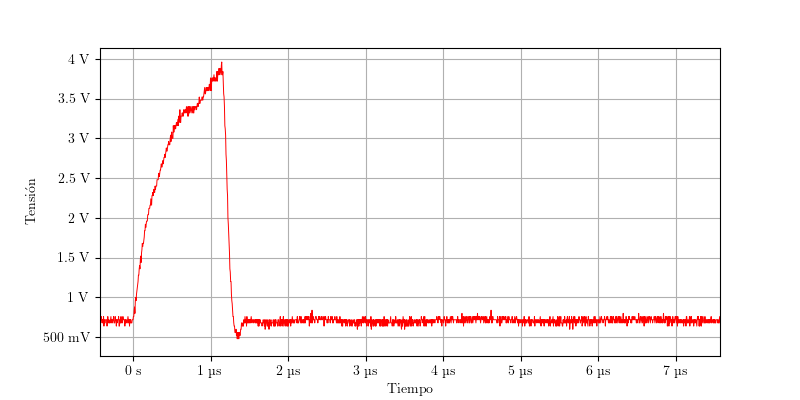
\includegraphics[width=\textwidth]{images/capturas-osciloscopio/TL494/pwm_vout_sin_bjt.png}
%     \caption{Tensión a la salida del TL494 sin colocar la etapa intermedia de ganancia de corriente}
%     \label{fig:pwm_vout_sin_bjt}
% \end{figure}

% 1) Corriente sin la etapa 
% DONE

% 2) Corriente de entrada y de salida con la etapa

% 3) Tensión a la salida sin la etapa
% DONE

% 3) Tensión a la salida con la etapa
% DONE

% Hay que ver eso de las oscilaciones en la corriente

\subsection{Driver}

%En la figura \ref{fig:driver_expected_waveforms} se muestran algunas formas de onda del circuito del driver con las que se hicieron comparaciones para verificar su correcto funcionamiento.

%\begin{figure}[H]
%    \centering
%    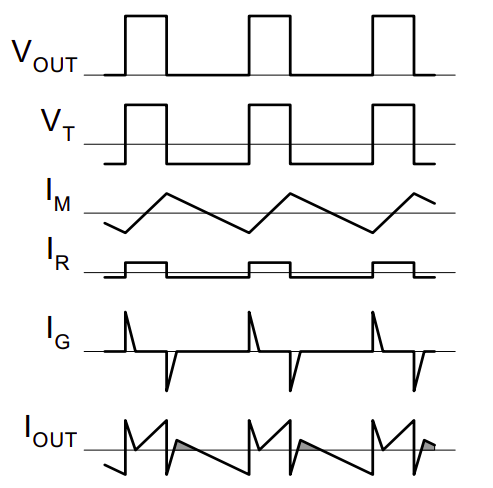
\includegraphics[width=0.7\textwidth]{images/driver_expected_waveforms.png}
%    \caption{Formas de onda esperadas de distintas señales del driver \cite{gatedrivers}}
%    \label{fig:driver_expected_waveforms}
%\end{figure}

% 1) Tensiones en el transformador de señal 

    % Forma de onda: Rectangular 
    % Amplitud: -Vc a Vdrv-Vc 
    % Son iguales dada la relación 1:1 del transformador. 
    
En la figura \ref{fig:osc:7} se muestra la tensión en el primario del transformador. 
La forma de la señal presenta una gran distorsión respecto a la rectangular esperada según la nota de aplicación \cite{gatedrivers}.
A pesar de ello, coincide en forma aproximada con la señal simulada, tanto en forma como en amplitud, de la figura \ref{fig:sim:4}.

Dado que es la primera señal de tensión del driver, la situación descripta anteriormente se reproduce en las siguientes formas de onda, como lo son la tensión en el secundario de la figura \ref{fig:osc:9}, la corriente por la resistencia entre gate y source de la figura \ref{fig:osc:13} y la tensión a la salida del driver de la figura \ref{fig:driver_vout_connected}.
Esta última señal es la que controla al MOSFET de lado alto (tensión entre \textit{gate} y \textit{source} del transistor) y presenta la oscilación no deseada de $f_{osc}=1.25MHz$.

\begin{figure}[H]
    \centering
    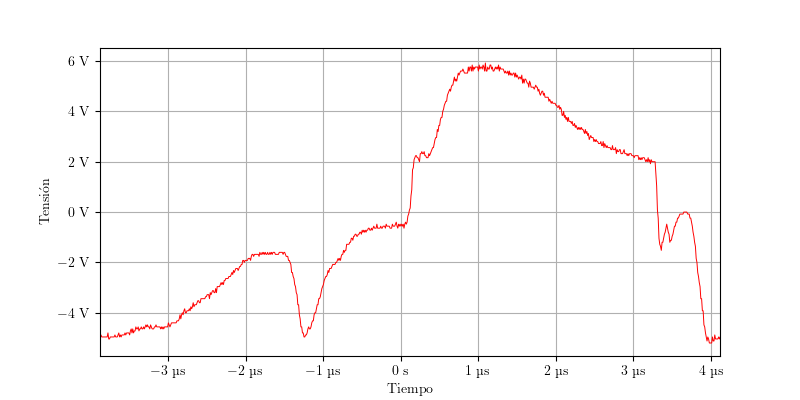
\includegraphics[width=0.9\textwidth]{images/capturas-osciloscopio/17-11-2022/7.png}
    \caption{Tensión en el primario del transformador del driver}
    \label{fig:osc:7}
\end{figure}

\begin{figure}[H]
    \centering
    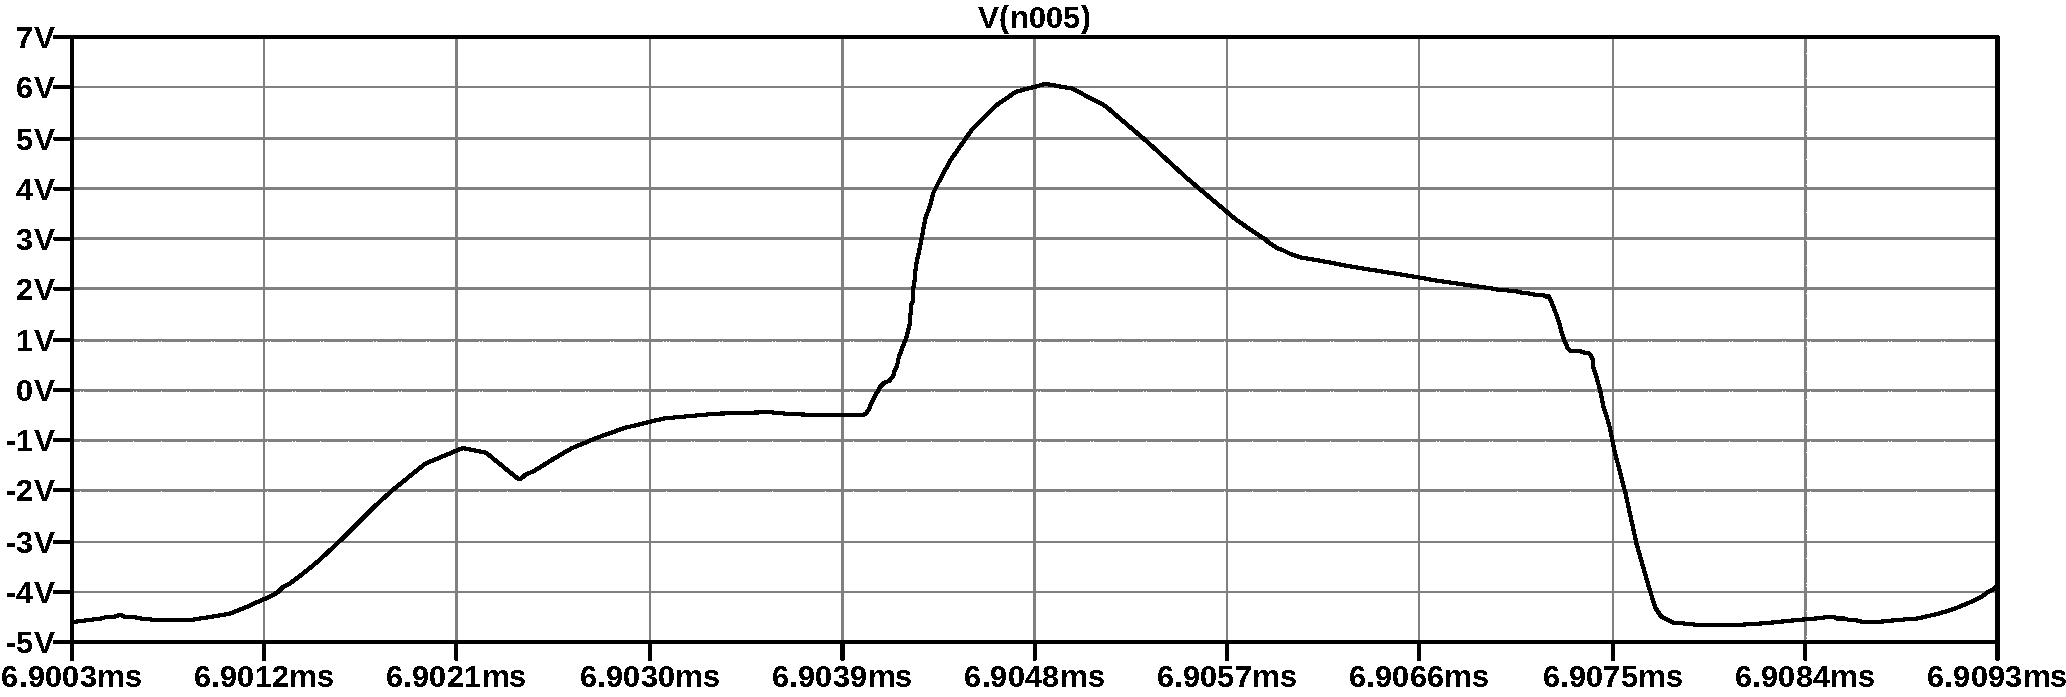
\includegraphics[width=\textwidth]{images/sim/4.pdf}
    \caption{Simulación de la tensión en el primario del transformador del driver}
    \label{fig:sim:4}
\end{figure}

\begin{figure}[H]
    \centering
    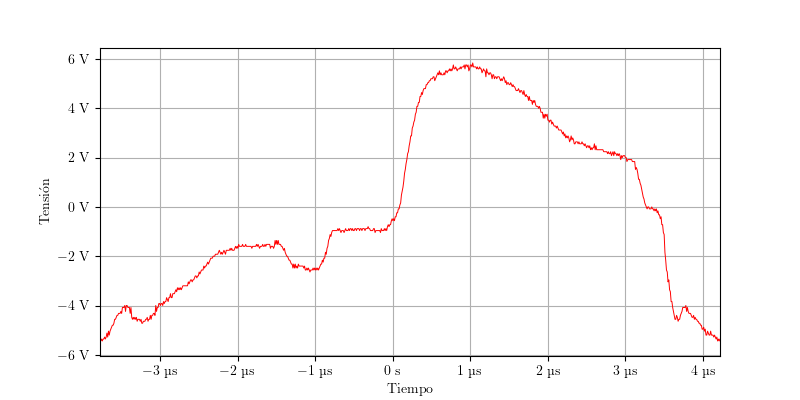
\includegraphics[width=0.9\textwidth]{images/capturas-osciloscopio/17-11-2022/9.png}
    \caption{Tensión en el secundario del transformador del driver}
    \label{fig:osc:9}
\end{figure}

\begin{figure}[H]
    \centering
    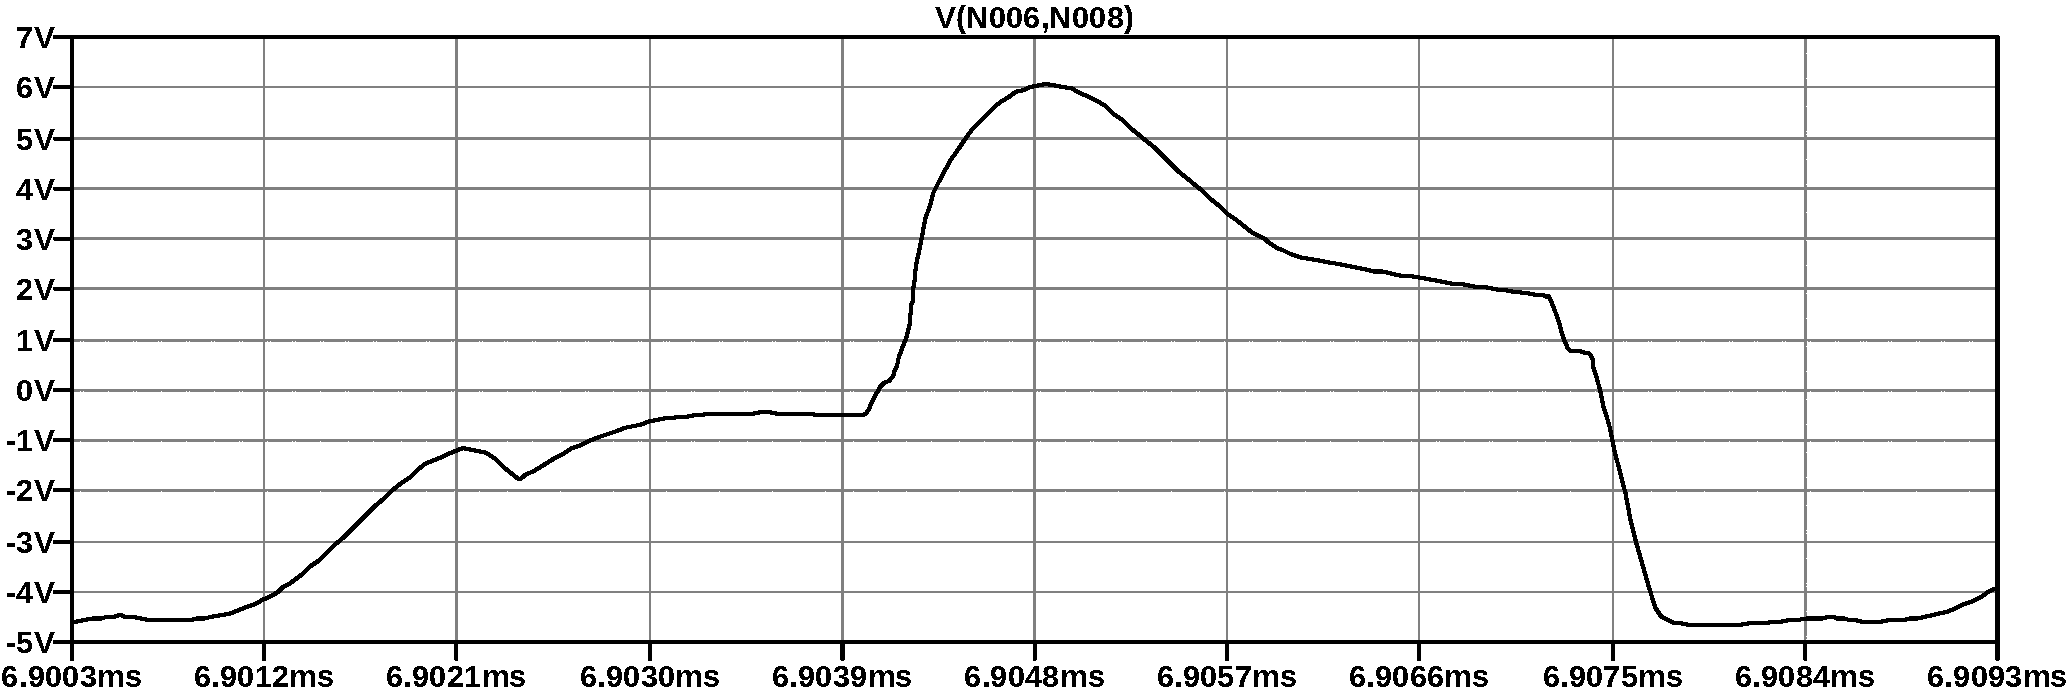
\includegraphics[width=\textwidth]{images/sim/5.pdf}
    \caption{Simulación de la tensión en el secundario del transformador del driver}
    \label{fig:sim:5}
\end{figure}

\begin{figure}[H]
    \centering
    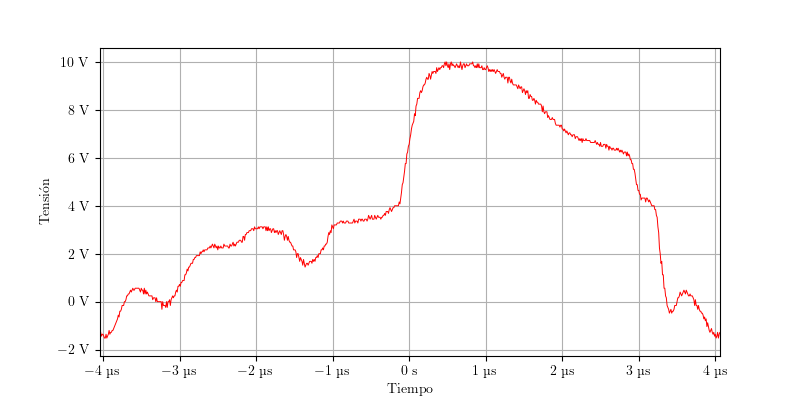
\includegraphics[width=\textwidth]{images/capturas-osciloscopio/17-11-2022/13.png}
    \caption{Corriente por la resistencia entre \textit{gate} y \textit{source} del MOSFET de lado alto}
    \label{fig:osc:13}
\end{figure}

\begin{figure}[H]
    \centering
    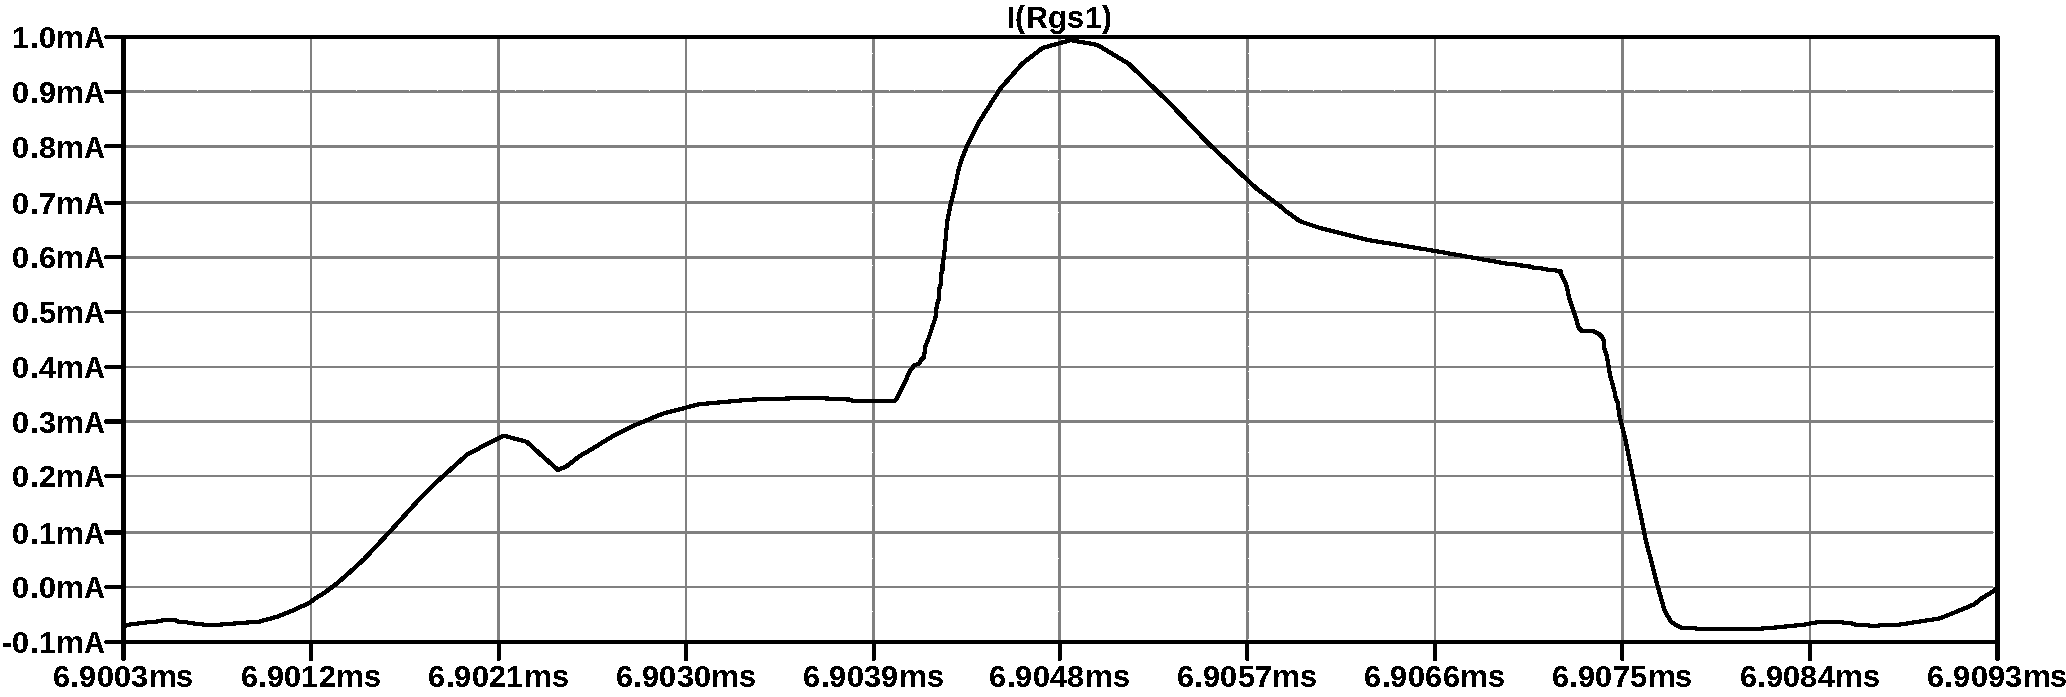
\includegraphics[width=\textwidth]{images/sim/7.pdf}
    \caption{Simulación de la corriente por la resistencia $R_{gs}$}
    \label{fig:sim:7}
\end{figure}

\begin{figure}[H]
    \centering
    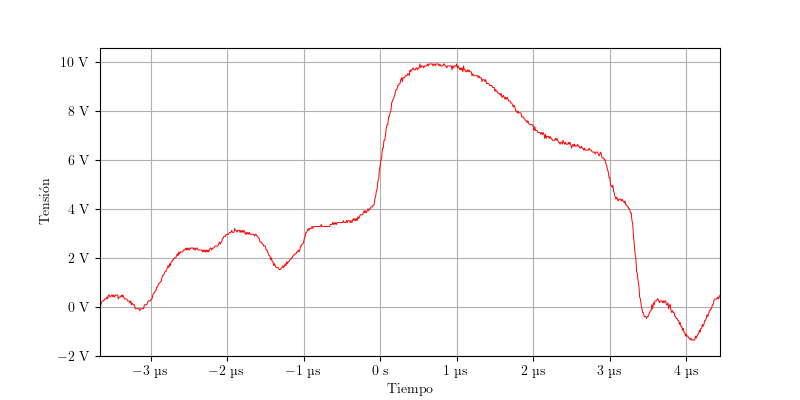
\includegraphics[width=\textwidth]{images/capturas-osciloscopio/17-11-2022/31.png} %Acá tuve que dejar la simulación vieja, porque la nueva está desfasada y esta hecha con otro D, queda mal
    \caption{Tensión a la salida del driver}
    \label{fig:driver_vout_connected}
\end{figure}

\begin{figure}[H]
    \centering
    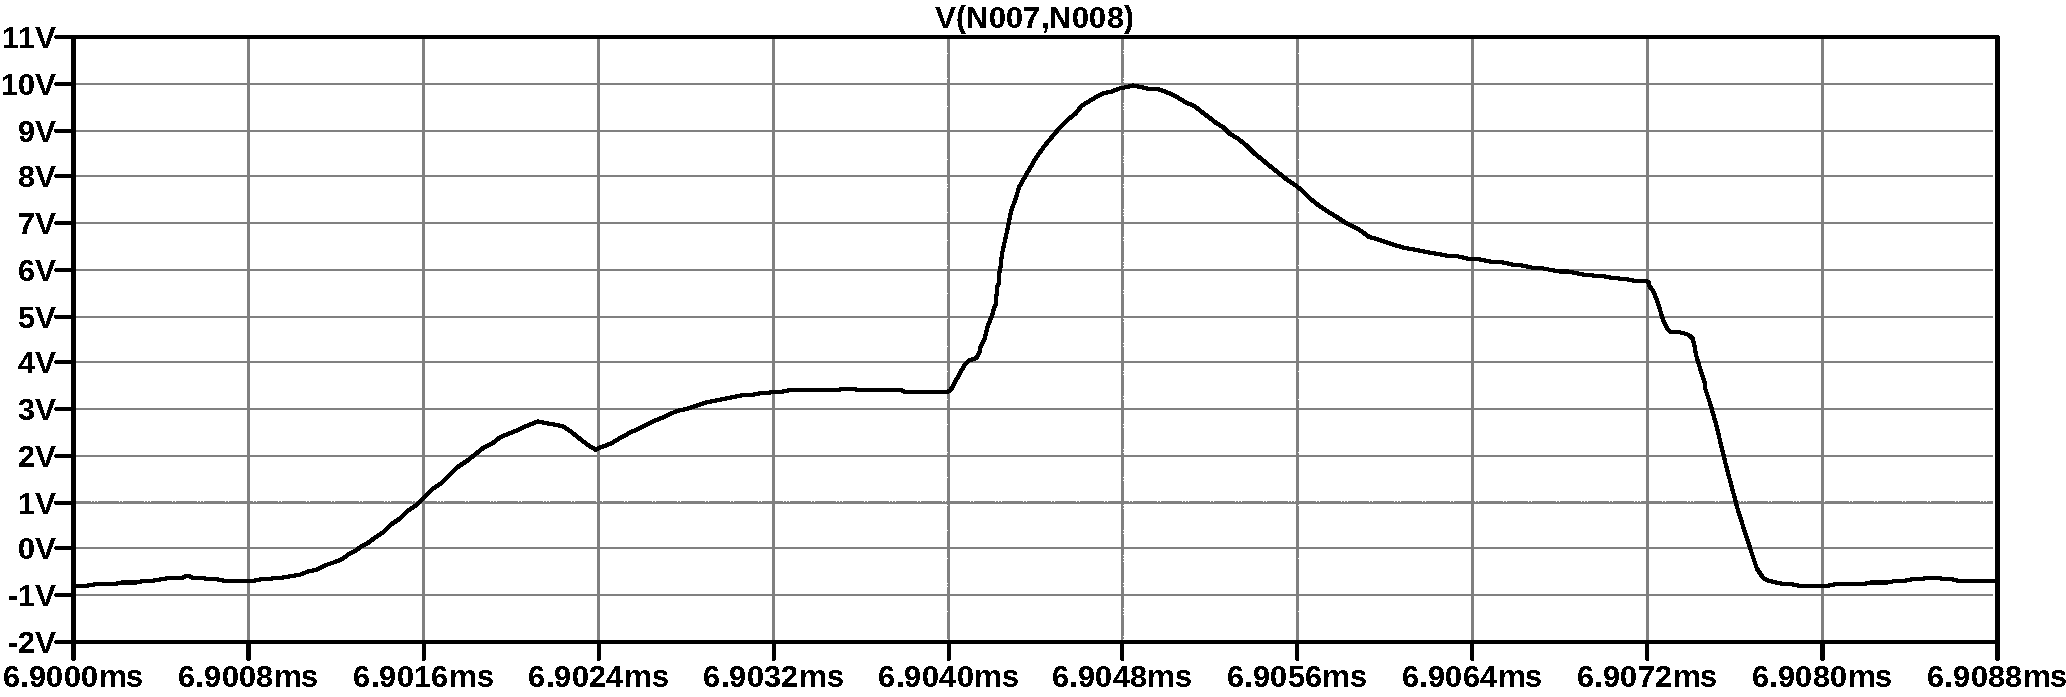
\includegraphics[width=\textwidth]{images/sim/15.pdf}
    \caption{Simulación de la tensión a la salida del driver}
    \label{fig:sim:driver_vout_connected}
\end{figure}

En la figura \ref{fig:osc:11} se muestra la corriente por el primario del transformador. La forma de onda presenta deformación y levemente mayor amplitud que la simulada de la figura \ref{fig:sim:6}.

\begin{figure}[H]
    \centering
    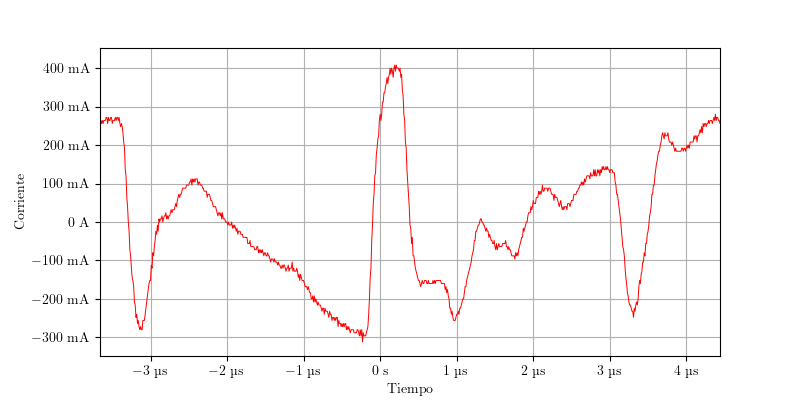
\includegraphics[width=\textwidth]{images/capturas-osciloscopio/17-11-2022/11.png}
    \caption{Corriente por el primario del transformador del driver}
    \label{fig:osc:11}
\end{figure}

\begin{figure}[H]
    \centering
    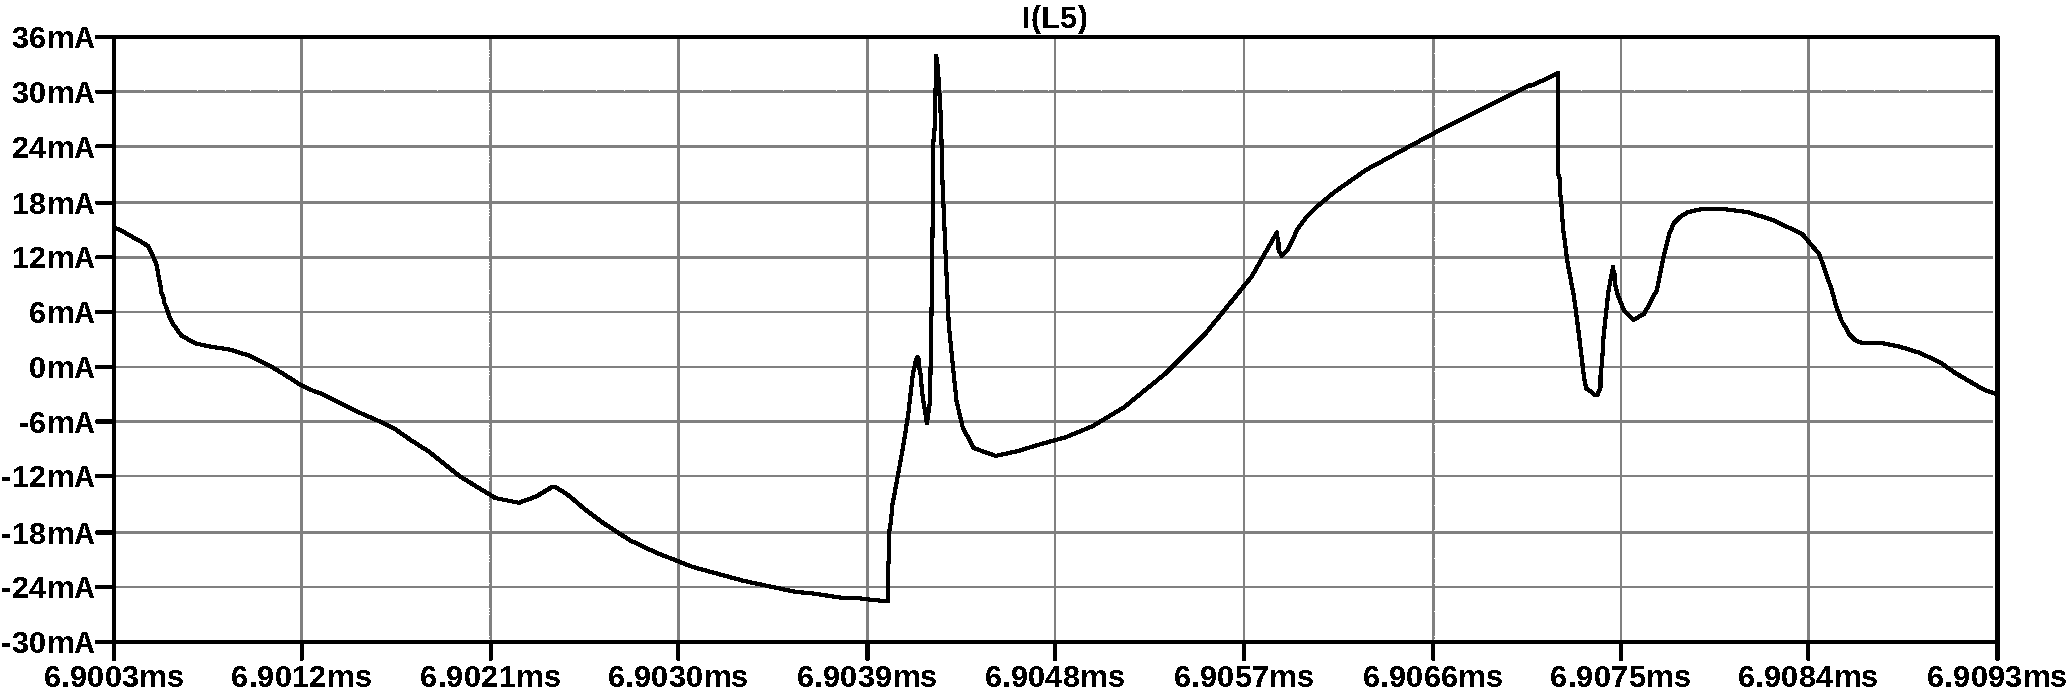
\includegraphics[width=\textwidth]{images/sim/6.pdf}
    \caption{Simulación de la corriente por el primario del transformador del driver}
    \label{fig:sim:6}
\end{figure}

% 2) Tensión Gate del MOSFET high side % Sería vout del driver?
% DONE

    % Forma de onda: Rectangular 
    % Amplitud: -Vd a Vdrv-Vd
    % Vd: Tensión en el diodo del secundario

% 3) Corriente de salida % FALTA MEDIR LAS CORRIENTES CON LA PCB

    % Compuesta por:

    % A) Corriente magnetizante

        % Forma de onda: triangular
        % Se mide en la Rc del primario. 

    % B) Corriente por Rgs

        % Forma de onda: rectangular

    % C) Corriente por Gate

        % Forma de onda: diente de sierra invertida y espejada con tiempo muerto 

\subsection{Convertidor}

\subsubsection{MOSFETs}

% 1) Vgs de ambos MOSFETs %Ya se midió en otros lados

% 2) Vds de ambos MOSFETs

En las figuras \ref{fig:vds_high} y \ref{fig:vds_low} se muestran las tensiones en los terminales \textit{drain} y \textit{source} de los MOSFETs del convertidor forward doble switch.
Exceptuando el sobrepico inicial y la oscilación de $f_{osc}=1.25MHz$, las señales coinciden con las simuladas de las figuras \ref{fig:vds_simulation_high} y \ref{fig:vds_simulation_low}. 

\begin{figure}[H]
    \centering
    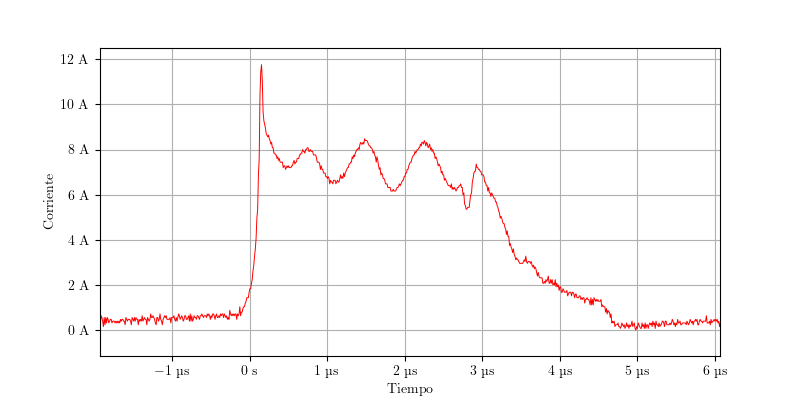
\includegraphics[width=0.9\textwidth]{images/capturas-osciloscopio/17-11-2022/33.png}
    \caption{Tensión $V_{DS}$ en el MOSFET de lado alto}
    \label{fig:vds_high}
\end{figure}

\begin{figure}[H]
    \centering
    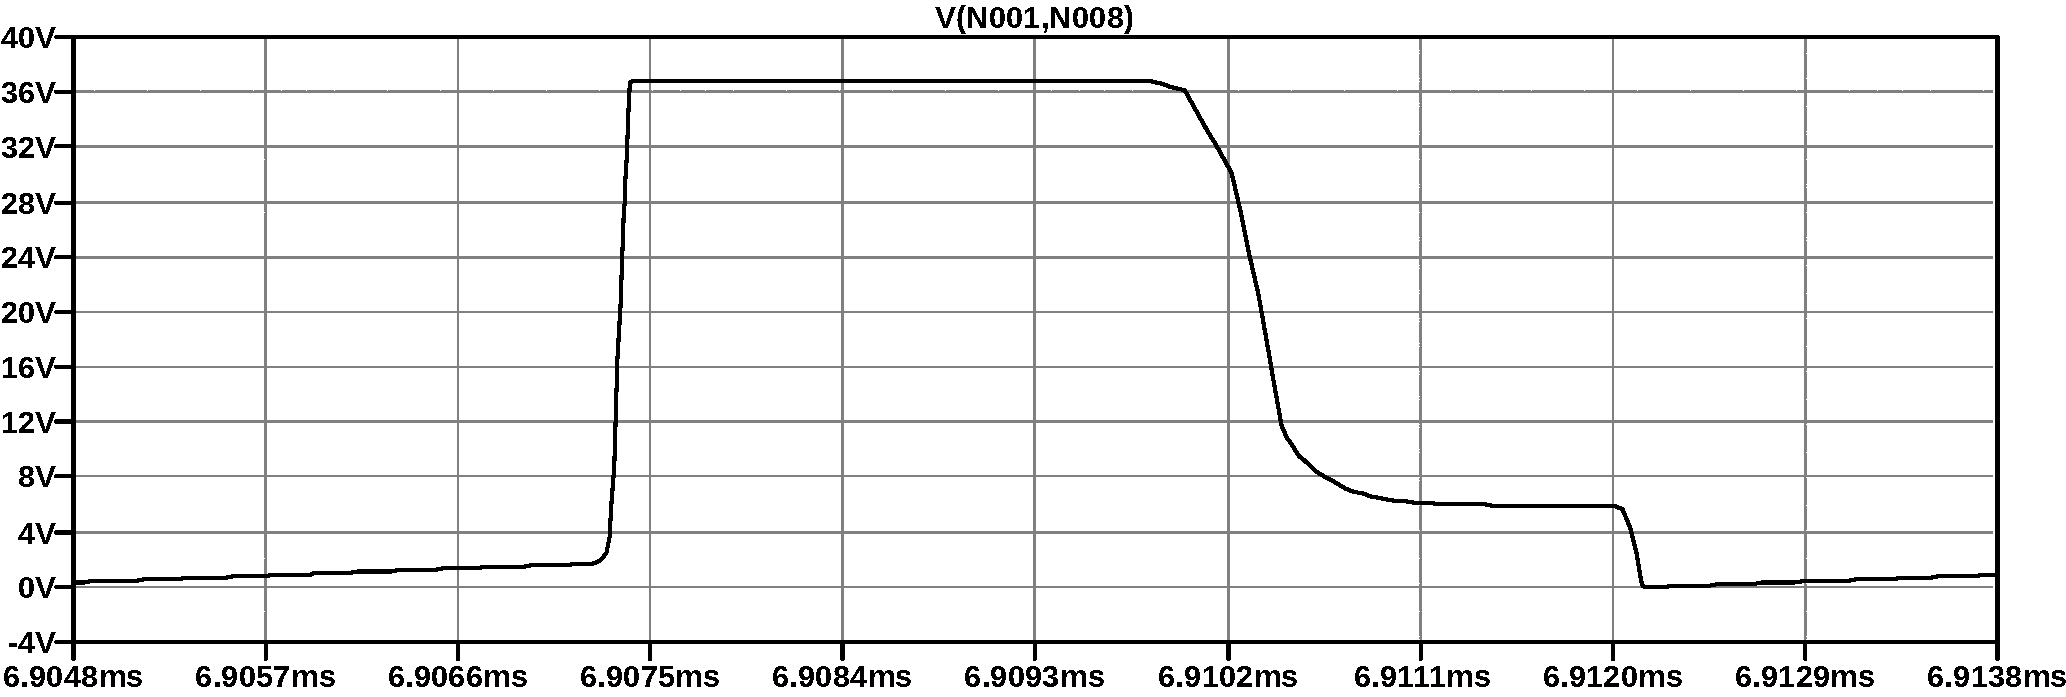
\includegraphics[width=\textwidth]{images/sim/16.pdf}
    \caption{Tensión $V_{DS}$ en el MOSFET de lado alto simulado en LTspice}
    \label{fig:vds_simulation_high}
\end{figure}

\begin{figure}[H]
    \centering
    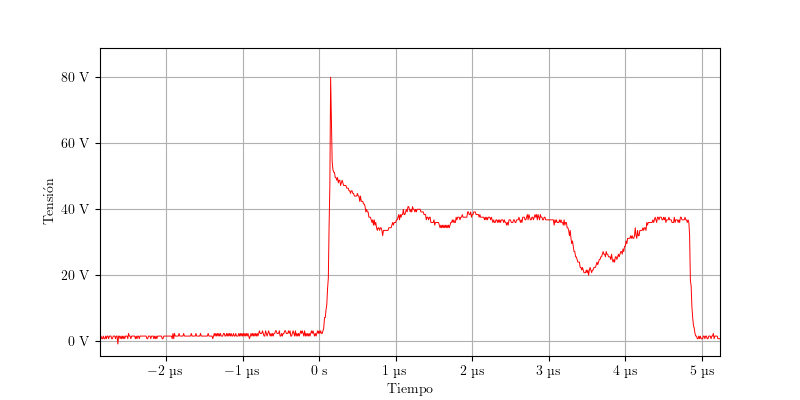
\includegraphics[width=0.9\textwidth]{images/capturas-osciloscopio/17-11-2022/36.png}
    \caption{Tensión $V_{DS}$ en el MOSFET de lado bajo}
    \label{fig:vds_low}
\end{figure}

\begin{figure}[H]
    \centering
    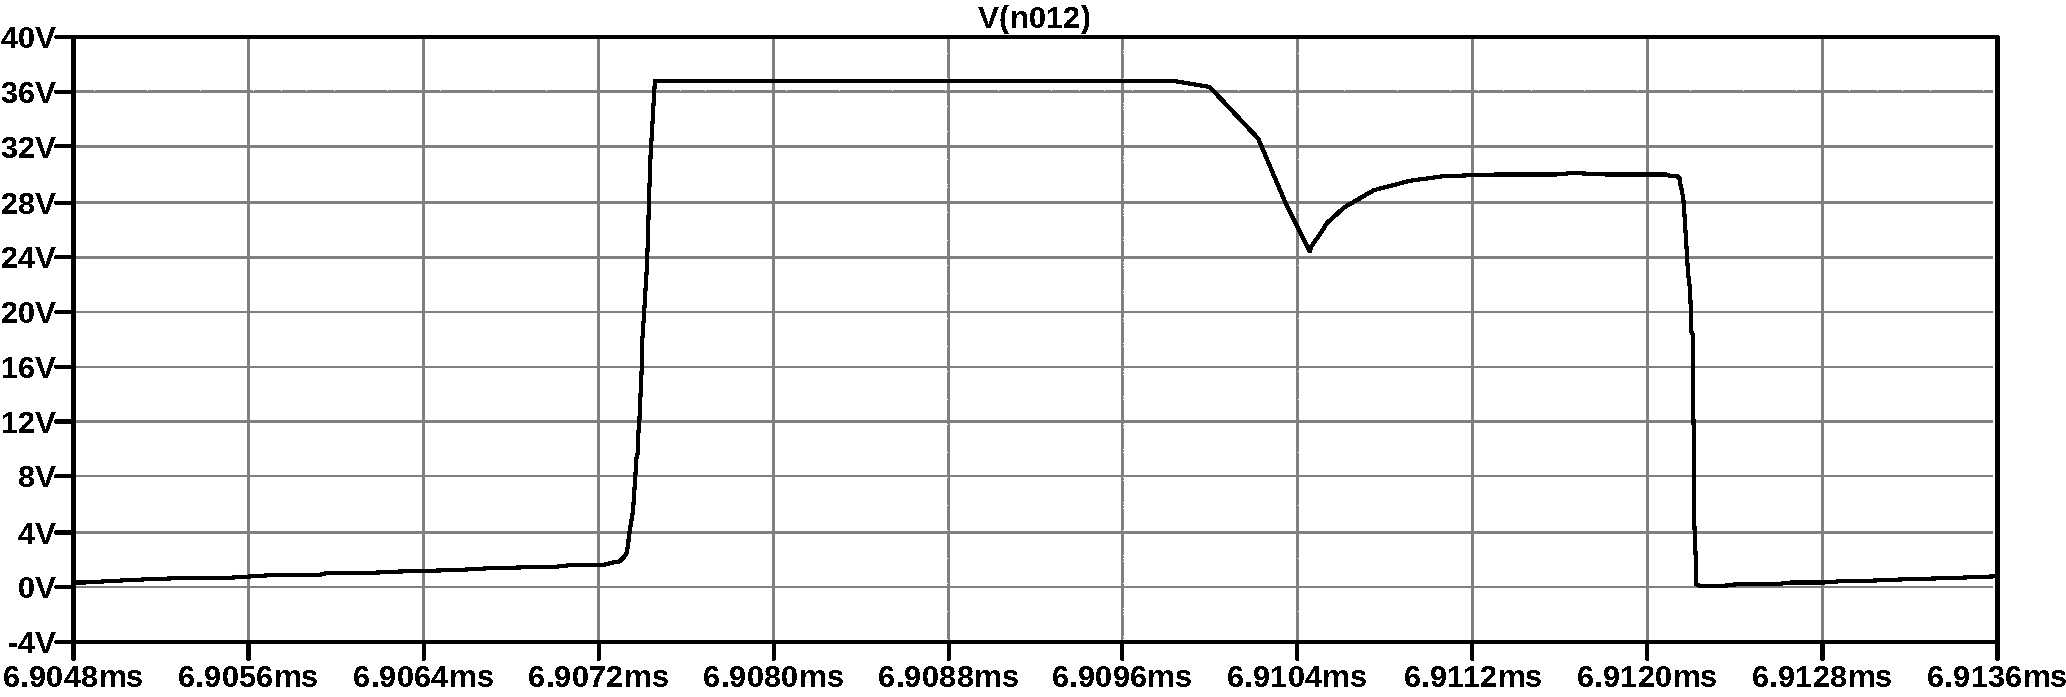
\includegraphics[width=\textwidth]{images/sim/18.pdf}
    \caption{Tensión $V_{DS}$ en el MOSFET de lado bajo simulado en LTspice}
    \label{fig:vds_simulation_low}
\end{figure}

% 3) Idrain de ambos MOSFETs

En las figuras \ref{fig:osc:20} y \ref{fig:osc:22} puede observarse la corriente por el terminal \textit{drain} de los MOSFETs del convertidor.
A partir de estas mediciones, las formas de onda de corriente no presentan componente continua ya que se utilizaron las puntas de corriente. En consecuencia, en las comparaciones se analizarán las formas de onda y las posibles oscilaciones.  
Si bien la forma de onda es triangular, respecto a las simulaciones de las figuras \ref{fig:sim:10} y \ref{fig:sim:11}, la amplitud obtenida es mucho menor. 
Además se percibe un sobrepico negativo en el flanco de bajada del MOSFET de lado bajo. 

\begin{figure}[H]
    \centering
    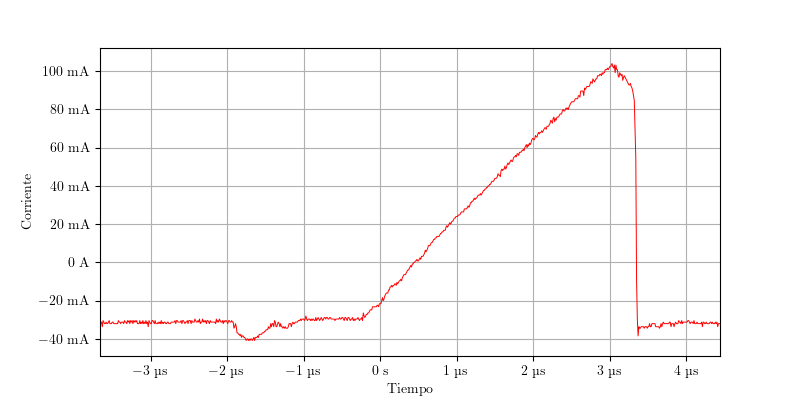
\includegraphics[width=0.8\textwidth]{images/capturas-osciloscopio/17-11-2022/20.png}
    \caption{Corriente que circula por el \textit{drain} del MOSFET de lado alto}
    \label{fig:osc:20}
\end{figure}

\begin{figure}[H]
    \centering
    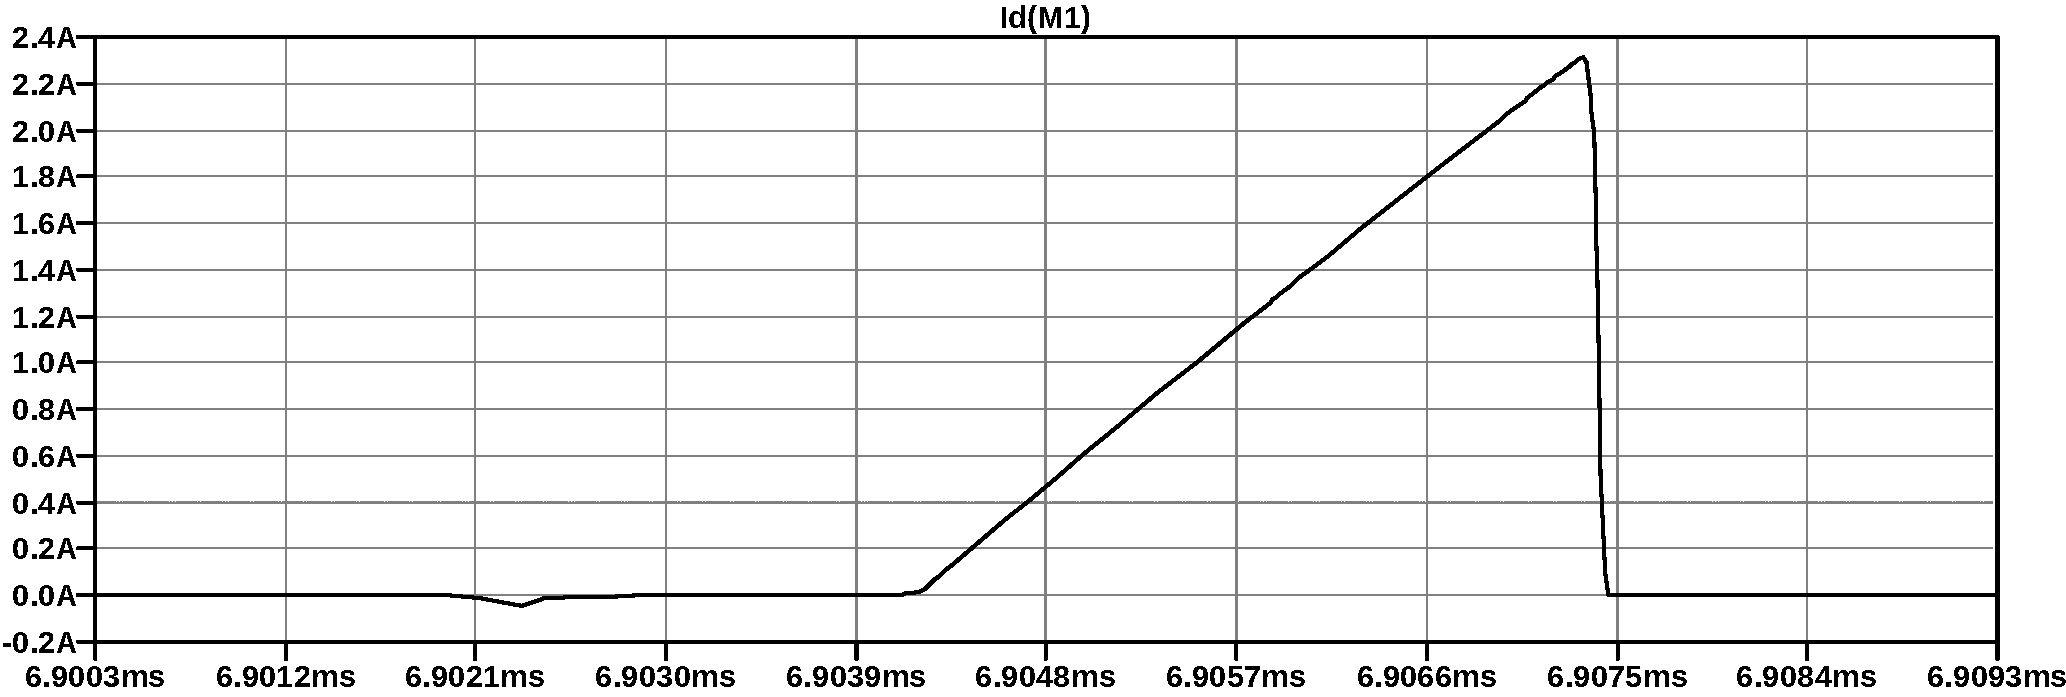
\includegraphics[width=\textwidth]{images/sim/10.pdf}
    \caption{Simulación de la corriente que circula por el \textit{drain} del MOSFET de lado alto}
    \label{fig:sim:10}
\end{figure} 

\begin{figure}[H]
    \centering
    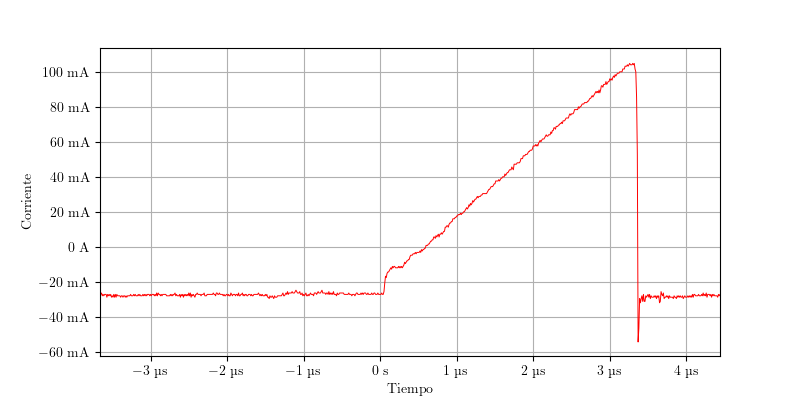
\includegraphics[width=0.8\textwidth]{images/capturas-osciloscopio/17-11-2022/22.png}
    \caption{Corriente que circula por el \textit{drain} del MOSFET de lado bajo}
    \label{fig:osc:22}
\end{figure}

\begin{figure}[H]
    \centering
    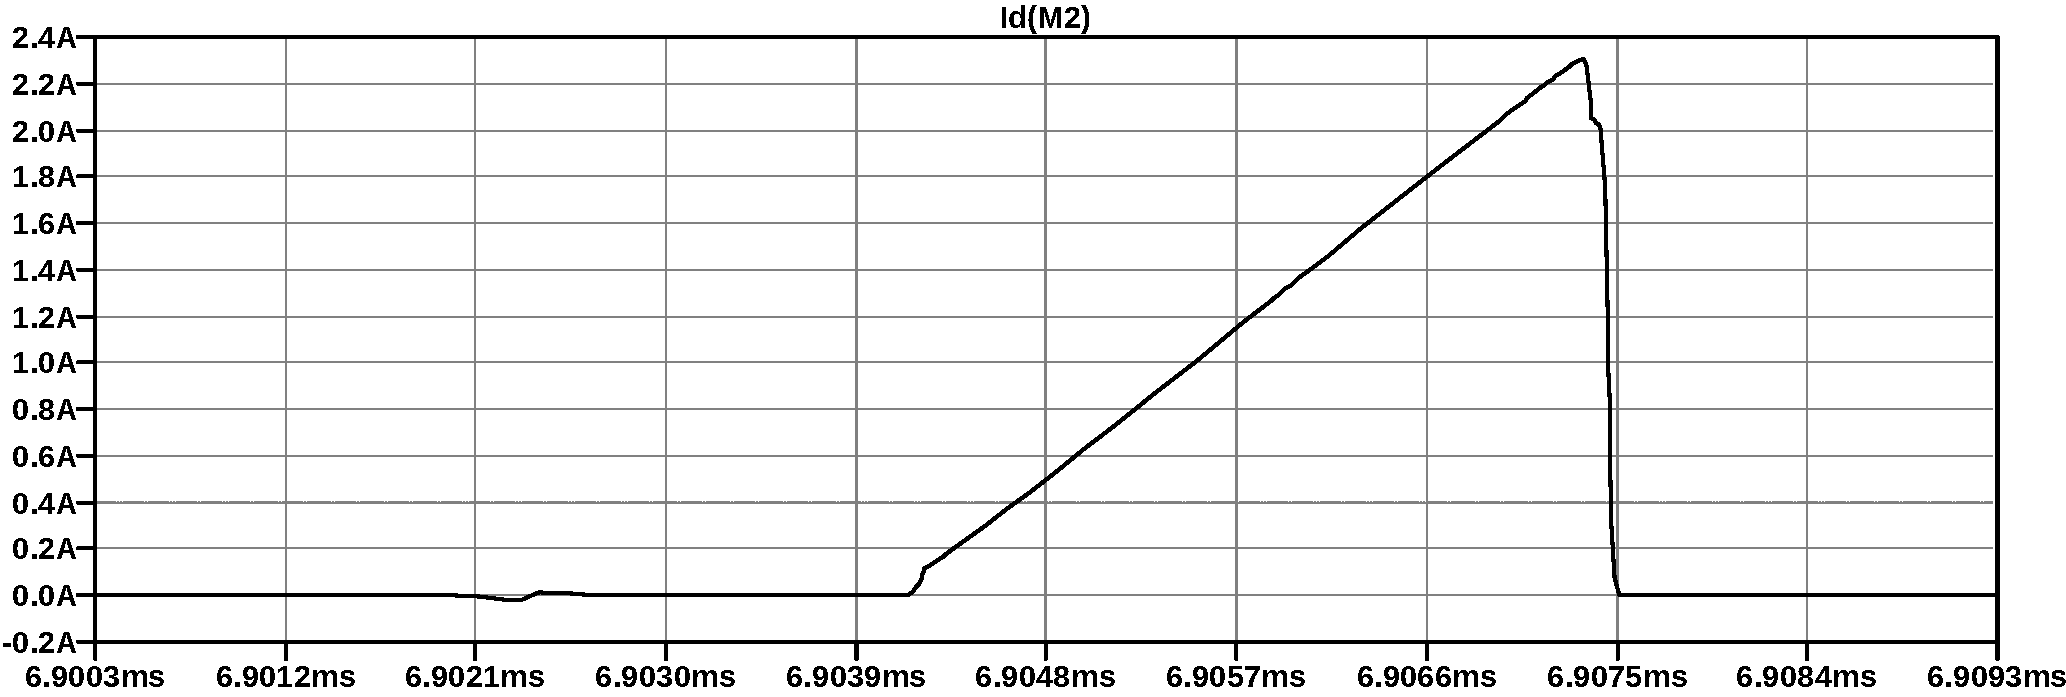
\includegraphics[width=\textwidth]{images/sim/11.pdf}
    \caption{Simulación de la corriente que circula por el \textit{drain} del MOSFET de lado bajo}
    \label{fig:sim:11}
\end{figure}

En las figuras \ref{fig:osc:15} y \ref{fig:osc:17} se muestra la corriente por el terminal \textit{gate} de los MOSFETs. Las formas de onda coinciden de forma aproximada con las simulaciones de las figuras \ref{fig:sim:8} y \ref{fig:sim:9}.

\begin{figure}[H]
    \centering
    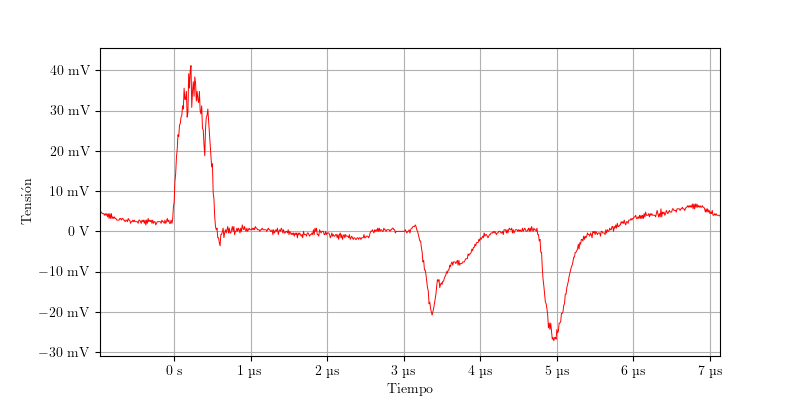
\includegraphics[width=0.8\textwidth]{images/capturas-osciloscopio/17-11-2022/15.png}
    \caption{Corriente que circula por el gate del MOSFET de lado alto}
    \label{fig:osc:15}
\end{figure}
 
\begin{figure}[H]
    \centering
    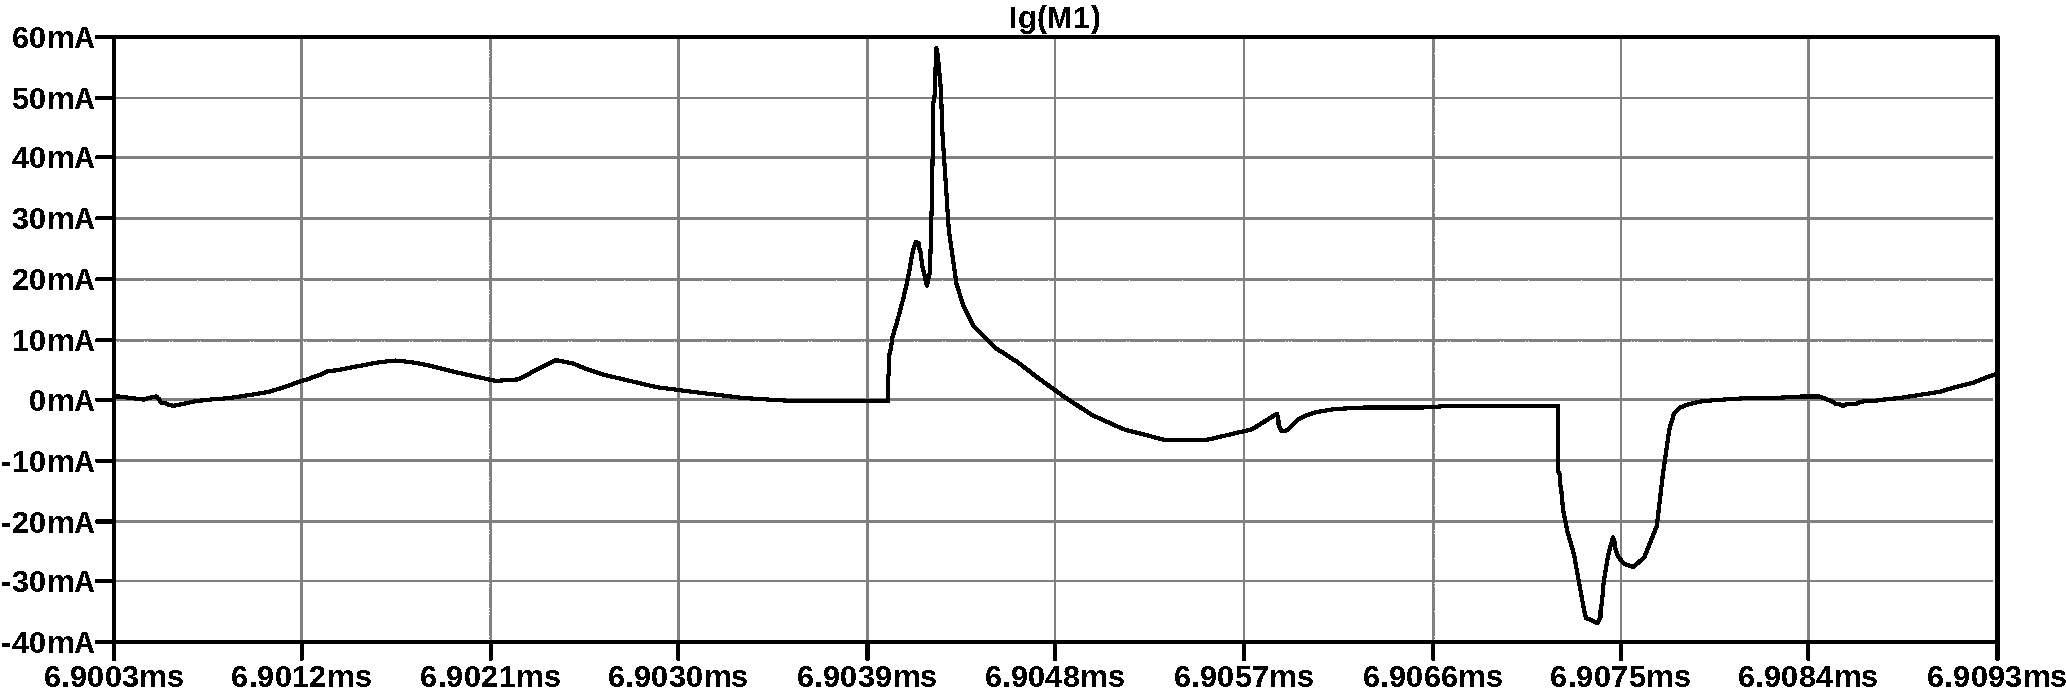
\includegraphics[width=\textwidth]{images/sim/8.pdf}
    \caption{Simulación de la corriente que circula por el gate del MOSFET de lado alto}
    \label{fig:sim:8}
\end{figure}
 
\begin{figure}[H]
    \centering
    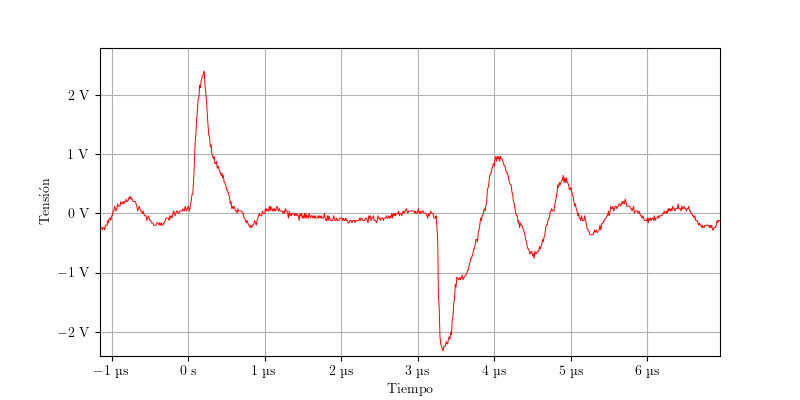
\includegraphics[width=0.8\textwidth]{images/capturas-osciloscopio/17-11-2022/17.png}
    \caption{Corriente que circula por el gate del MOSFET lado bajo}
    \label{fig:osc:17}
\end{figure}

\begin{figure}[H]
    \centering
    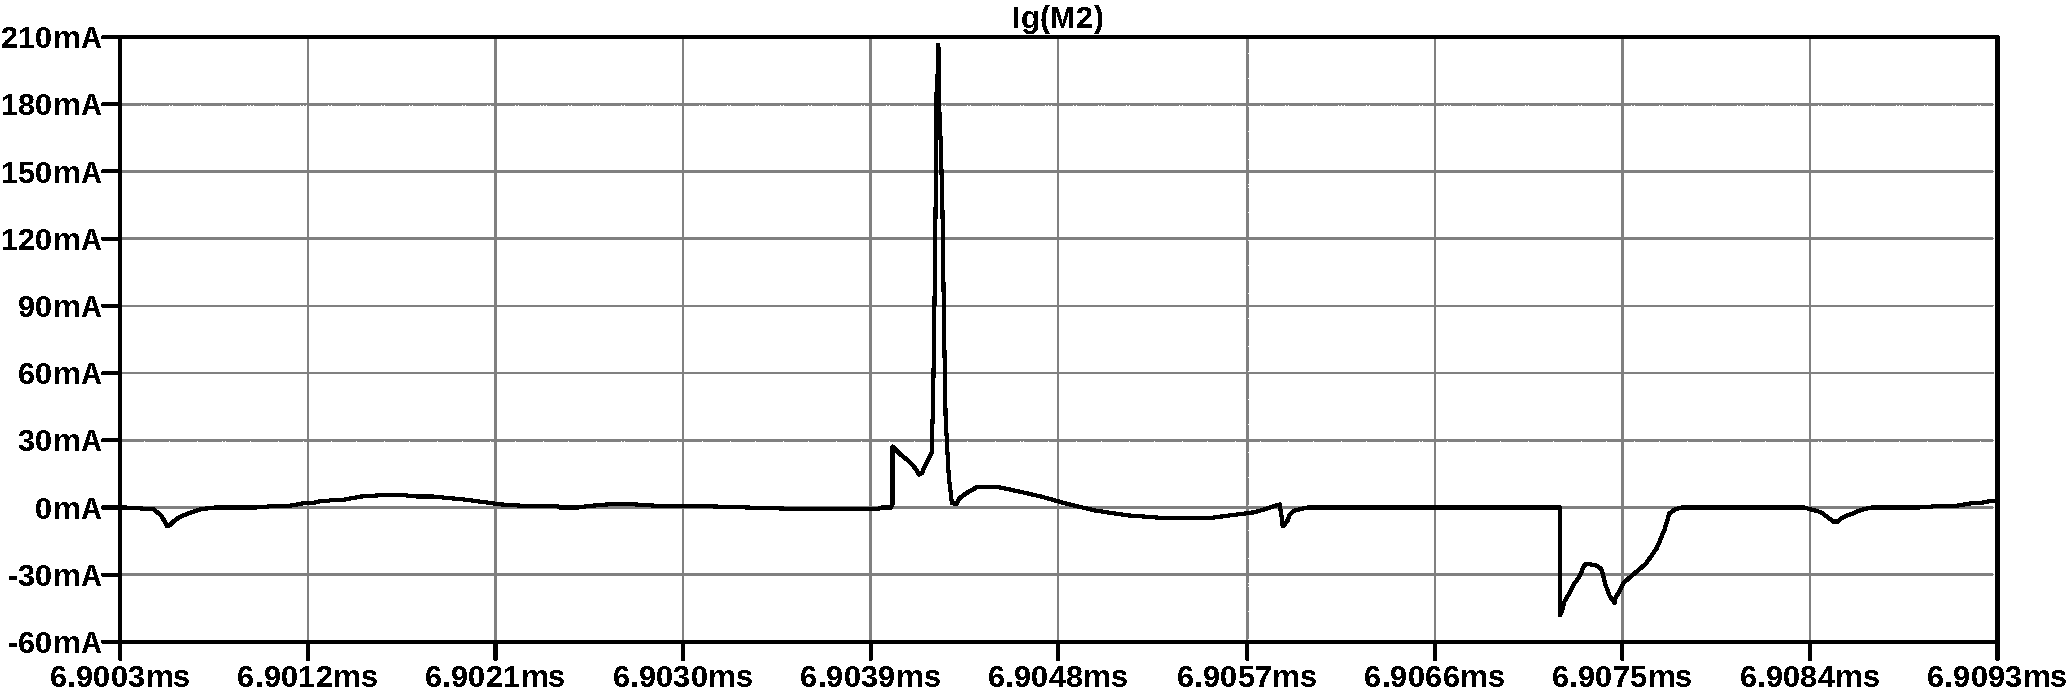
\includegraphics[width=\textwidth]{images/sim/9.pdf}
    \caption{Simulación de la corriente que circula por el gate del MOSFET de lado bajo}
    \label{fig:sim:9}
\end{figure}

\subsubsection{Transformador de potencia}
% 4) Tensiones en el E70

Las figuras \ref{fig:osc:38} y \ref{fig:osc:40} muestran las tensiones en el primario y el secundario del transformador de potencia. Puede observarse comparando con sus simulaciones (figuras \ref{fig:sim:19} y \ref{fig:sim:20}) que las oscilaciones son mucho mayores en el secundario del transformador.

\begin{figure}[H]
    \centering
    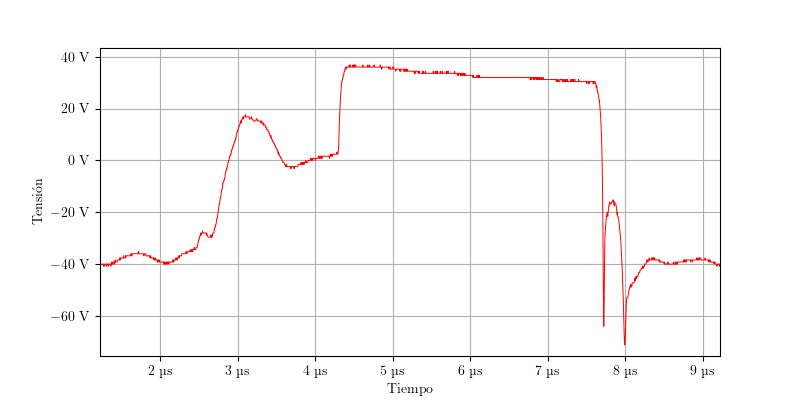
\includegraphics[width=0.8\textwidth]{images/capturas-osciloscopio/17-11-2022/55.png}
    \caption{Tensión en el primario del transformador de potencia}
    \label{fig:osc:38}
\end{figure}

\begin{figure}[H]
    \centering
    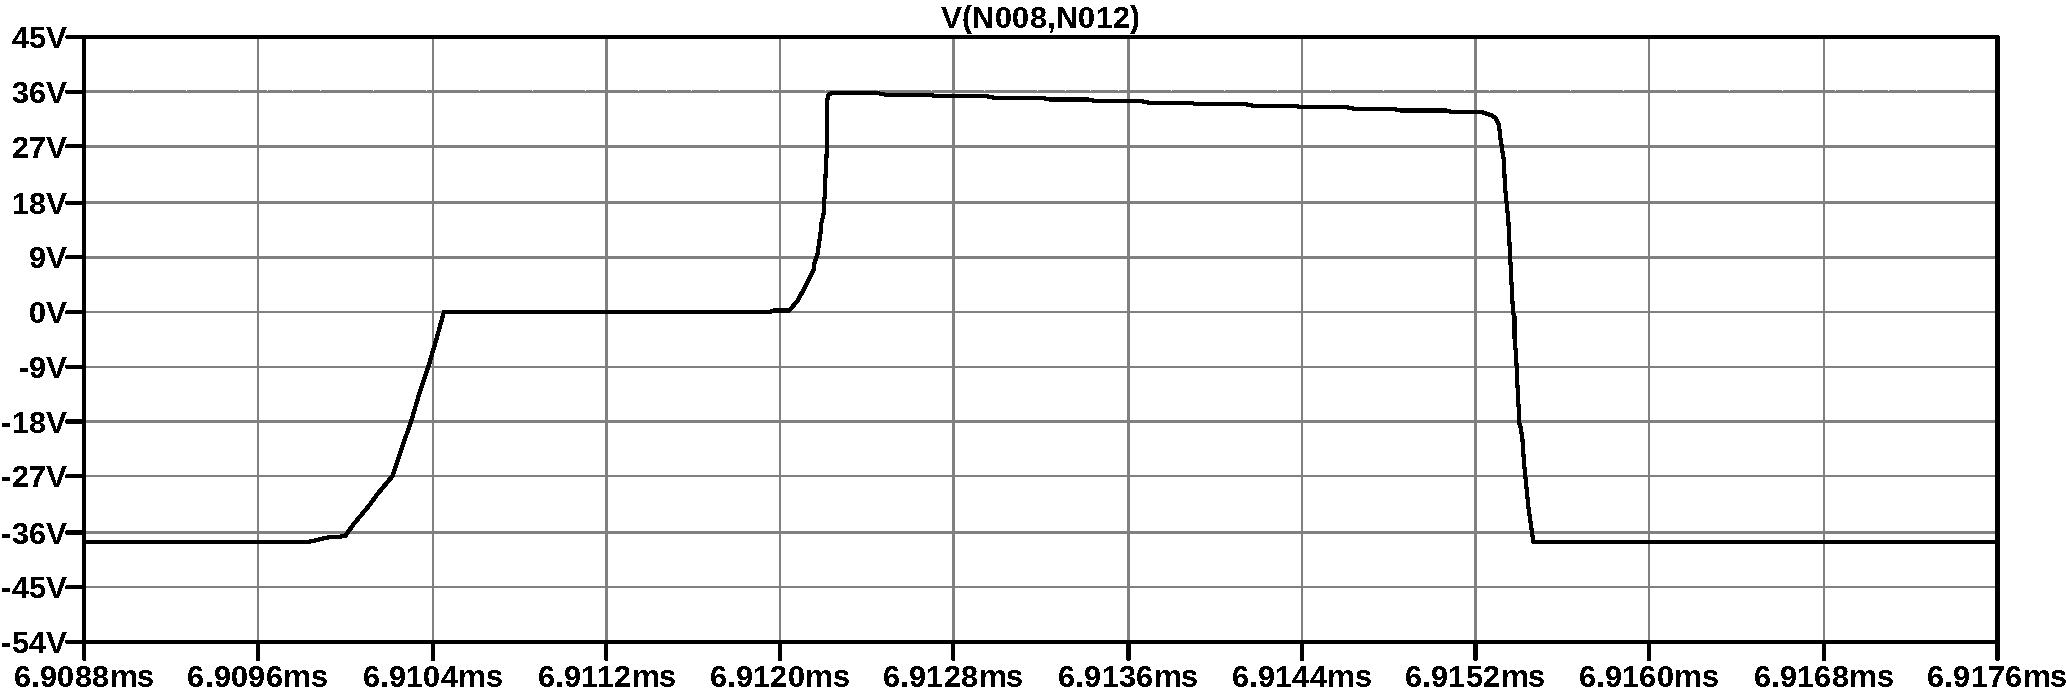
\includegraphics[width=\textwidth]{images/sim/19.pdf}
    \caption{Simulación de la tensión en el primario del transformador de potencia}
    \label{fig:sim:19}
\end{figure}

\begin{figure}[H]
    \centering
    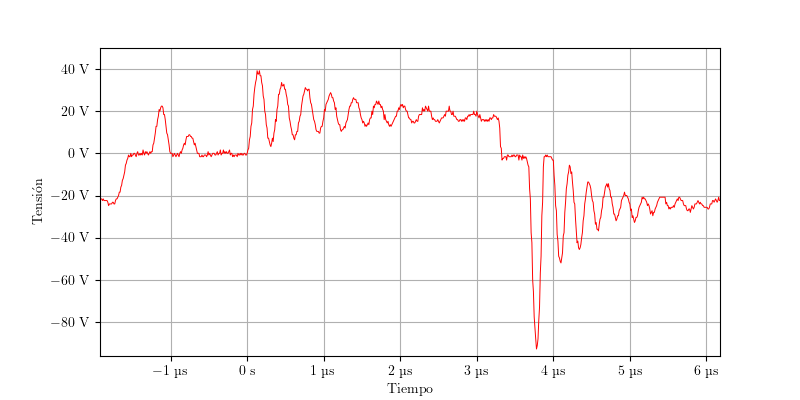
\includegraphics[width=0.8\textwidth]{images/capturas-osciloscopio/17-11-2022/40.png}
    \caption{Tensión en el secundario del transformador de potencia}
    \label{fig:osc:40}
\end{figure}

\begin{figure}[H]
    \centering
    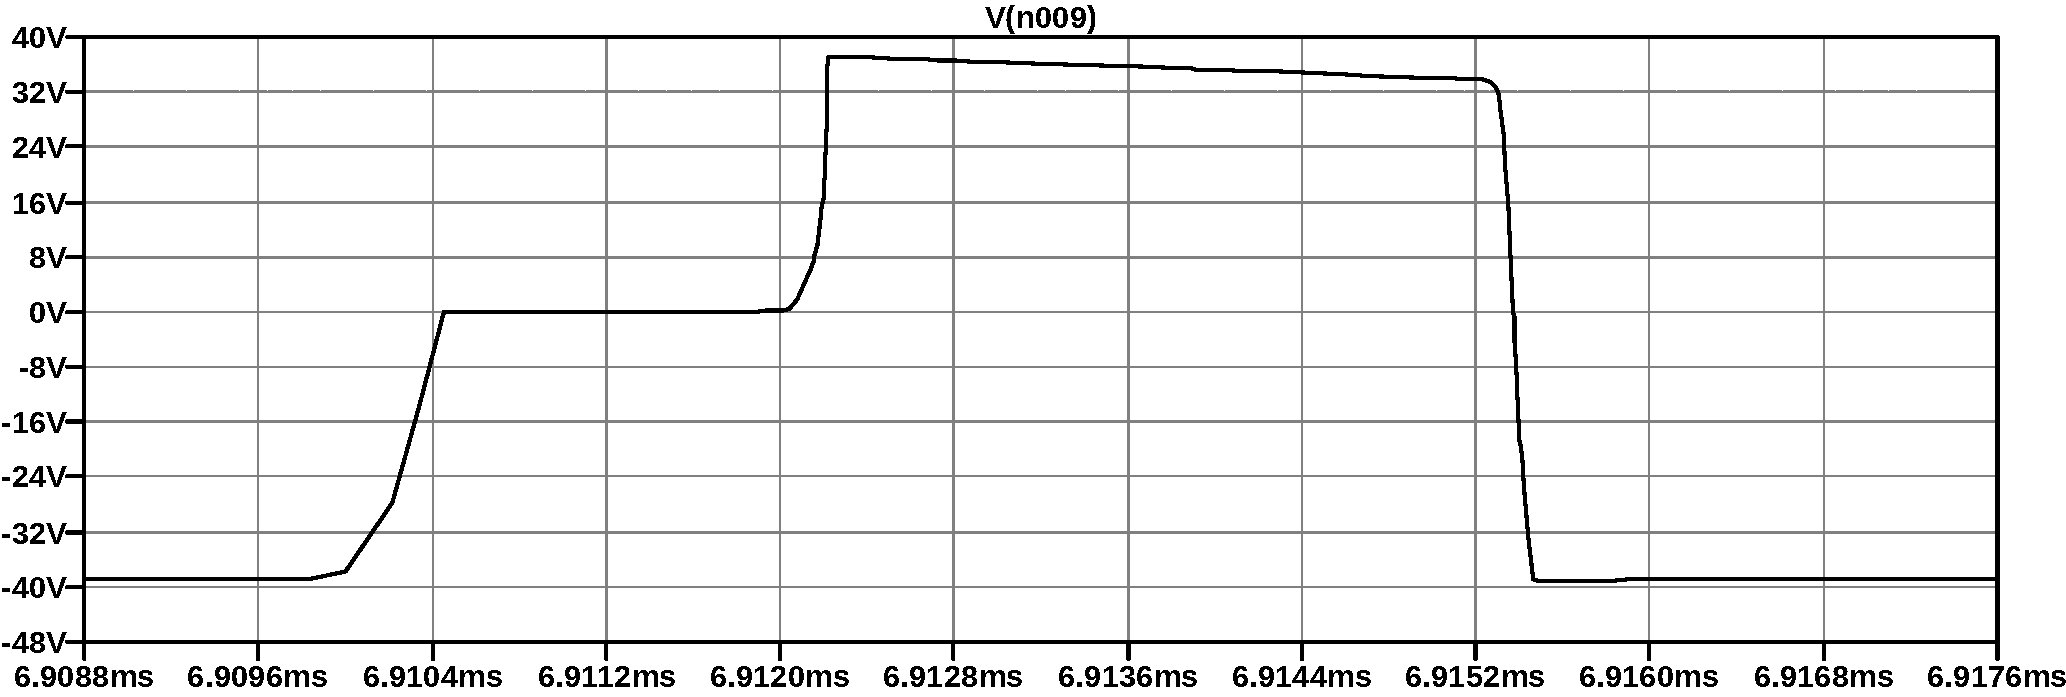
\includegraphics[width=\textwidth]{images/sim/20.pdf}
    \caption{Simulación de la tensión en el secundario del transformador de potencia}
    \label{fig:sim:20}
\end{figure}

Se observa que en el secundario del transformador, con una relación 1 a 1,
la tensión se ve reducida en gran medida.
Se ajustaron las vueltas del secundario para escalar a la tensión deseada.

\begin{figure}[H]
    \centering
    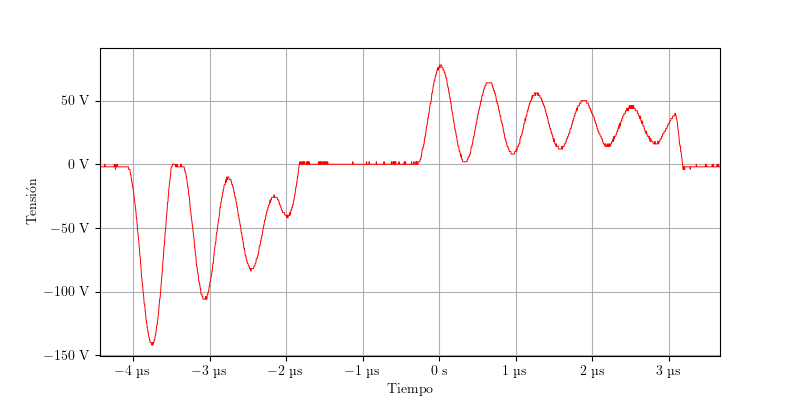
\includegraphics[width=0.8\textwidth]{images/capturas-osciloscopio/17-11-2022/56.png}
    \caption{Tensión en el secundario del transformador de potencia luego de ajustar la relación de vueltas del transformador a 2:1}
    \label{fig:osc:41}
\end{figure}

También puede observarse, comparándolo con la imagen anterior, que la señal pasa de una tensión de 36V a 0V,
y luego de 0V a -36V, mientras que con la relación original y en la simulación la tensión pasa de 36V a -36V directamente,
el cual es el comportamiento esperado.

% 5) Corriente en el primario %Del e70?

    % Medir la componente continua. IMPOSSIBLE
Las figuras \ref{fig:osc:24} muestra la corriente que circula por el primario del transformador de potencia. La figura \ref{fig:sim:12} muestra la simulación de la misma.

\begin{figure}[H]
    \centering
    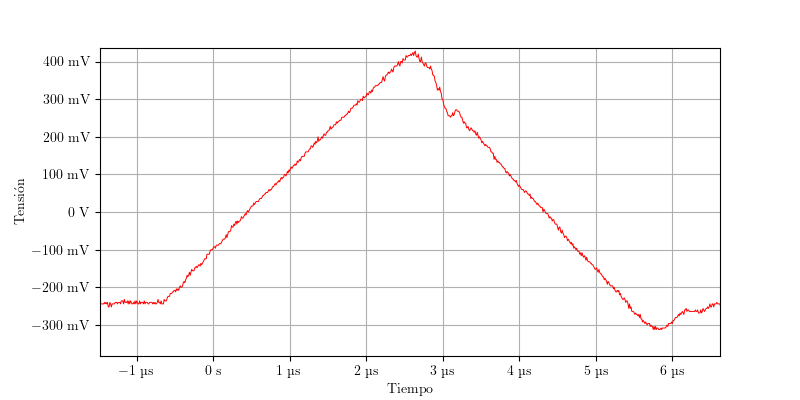
\includegraphics[width=0.8\textwidth]{images/capturas-osciloscopio/17-11-2022/24.png}
    \caption{Corriente en el primario del transformador de potencia}
    \label{fig:osc:24}
\end{figure}

\begin{figure}[H]
    \centering
    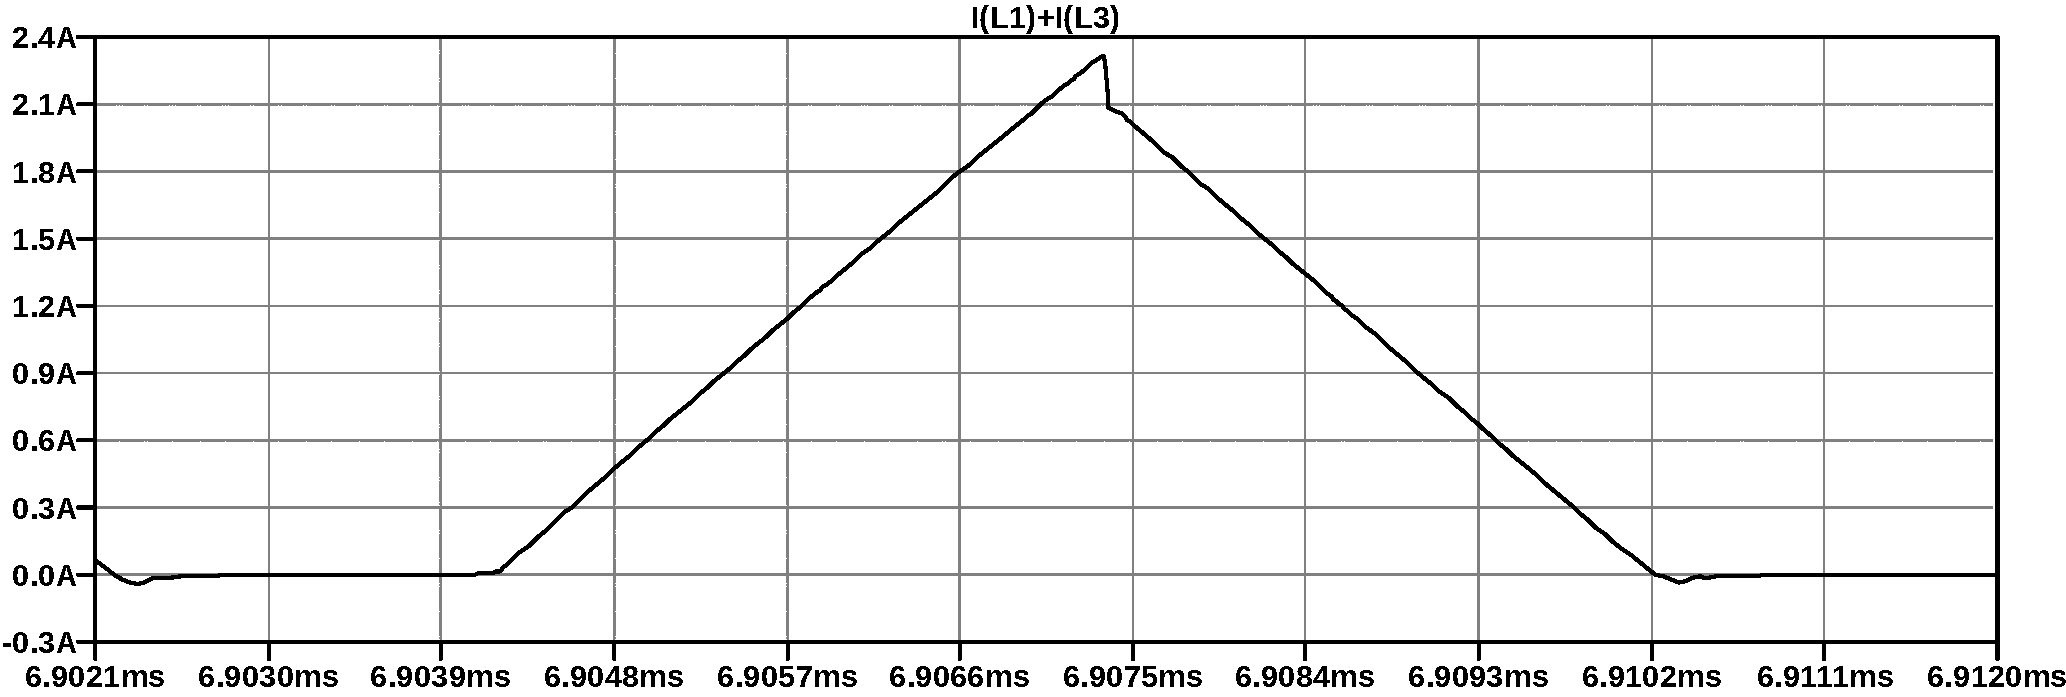
\includegraphics[width=\textwidth]{images/sim/12.pdf}
    \caption{Simulación de la corriente en el primario del transformador de potencia}
    \label{fig:sim:12}
\end{figure}

\subsubsection{Circuito de salida}
% 7) Corriente en el inductor junto con su ripple

La corriente por el inductor de salida se muestra en la figura \ref{fig:osc:66}. La figura \ref{fig:sim:13} muestra su simulación.

\begin{figure}[H]
    \centering
    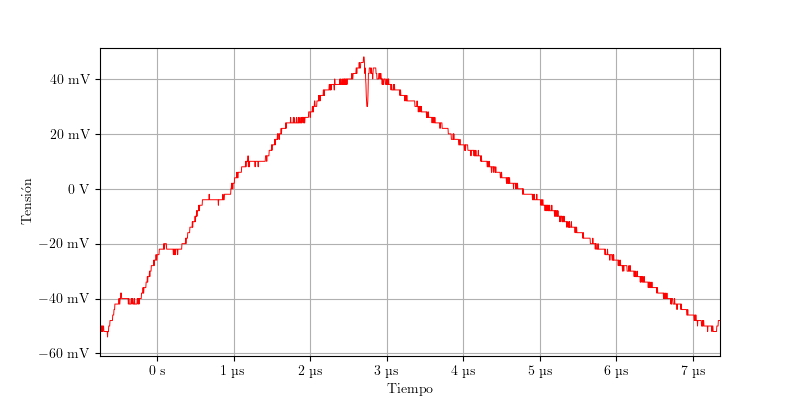
\includegraphics[width=0.8\textwidth]{images/capturas-osciloscopio/17-11-2022/66.png}
    \caption{Corriente en el inductor del filtro de salida}
    \label{fig:osc:66}
\end{figure}

\begin{figure}[H]
    \centering
    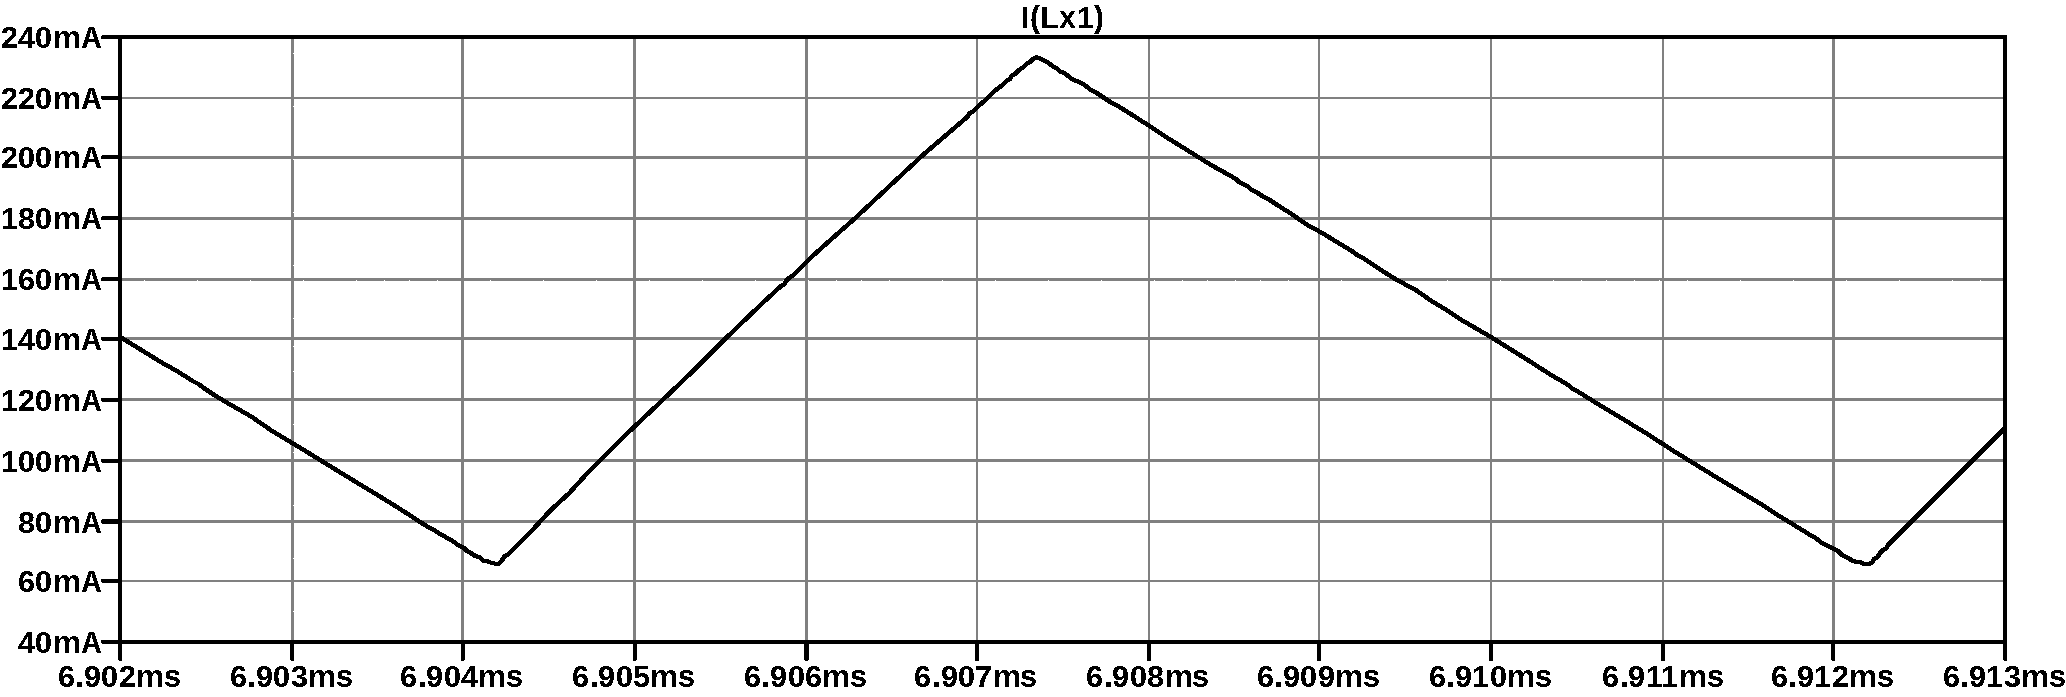
\includegraphics[width=\textwidth]{images/sim/13.pdf}
    \caption{Simulación de la corriente en el inductor del filtro de salida}
    \label{fig:sim:13}
\end{figure}

La amplitud de la forma de onda del prototipo es $30mA$ menor a la simulada. 
Además, presenta una oscilación de $f=3.68MHz$ en la rampa de subida y de $f=38.5MHz$ en la de bajada, la cual causa que la captura del osciloscopio se vea recortada. 

En las figuras \ref{fig:osc:67} y \ref{fig:sim:14ripple} se muestra la corriente por la resistencia de carga y su simulación, respectivamente. Se puede observar que el ripple obtenido es mayor al simulado.

La figura \ref{fig:sim:14} muestra la simulación de la corriente de salida durante el encendido.
% 8) Corriente de salida junto con su ripple 

    % Idealmente medir 1A-1.6A del modo elegido. 

\begin{figure}[H]
    \centering
    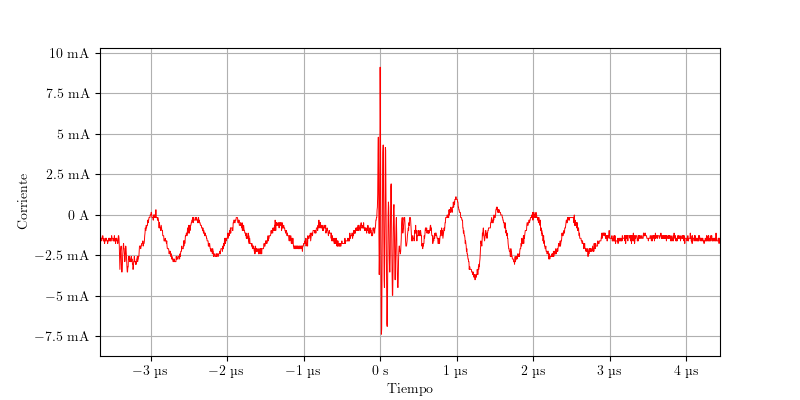
\includegraphics[width=0.8\textwidth]{images/capturas-osciloscopio/17-11-2022/67.png}
    \caption{Ripple de corriente por la carga}
    \label{fig:osc:67}
\end{figure}

\begin{figure}[H]
    \centering
    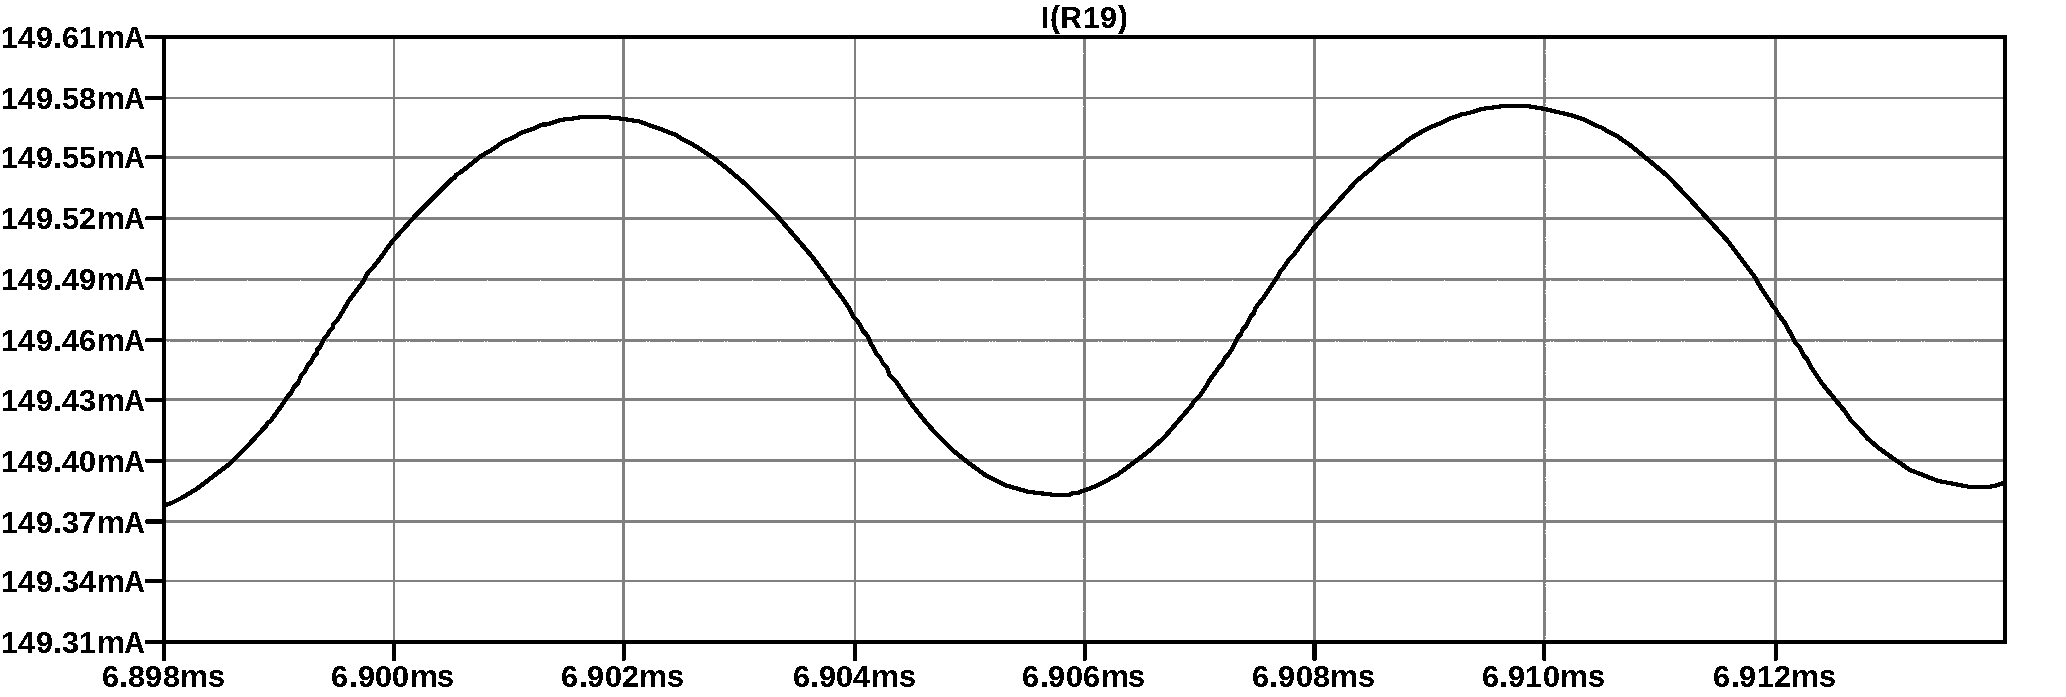
\includegraphics[width=\textwidth]{images/sim/14-ripple.pdf}
    \caption{Simulación del ripple de corriente por la carga}
    \label{fig:sim:14ripple}
\end{figure}

\begin{figure}[H]
    \centering
    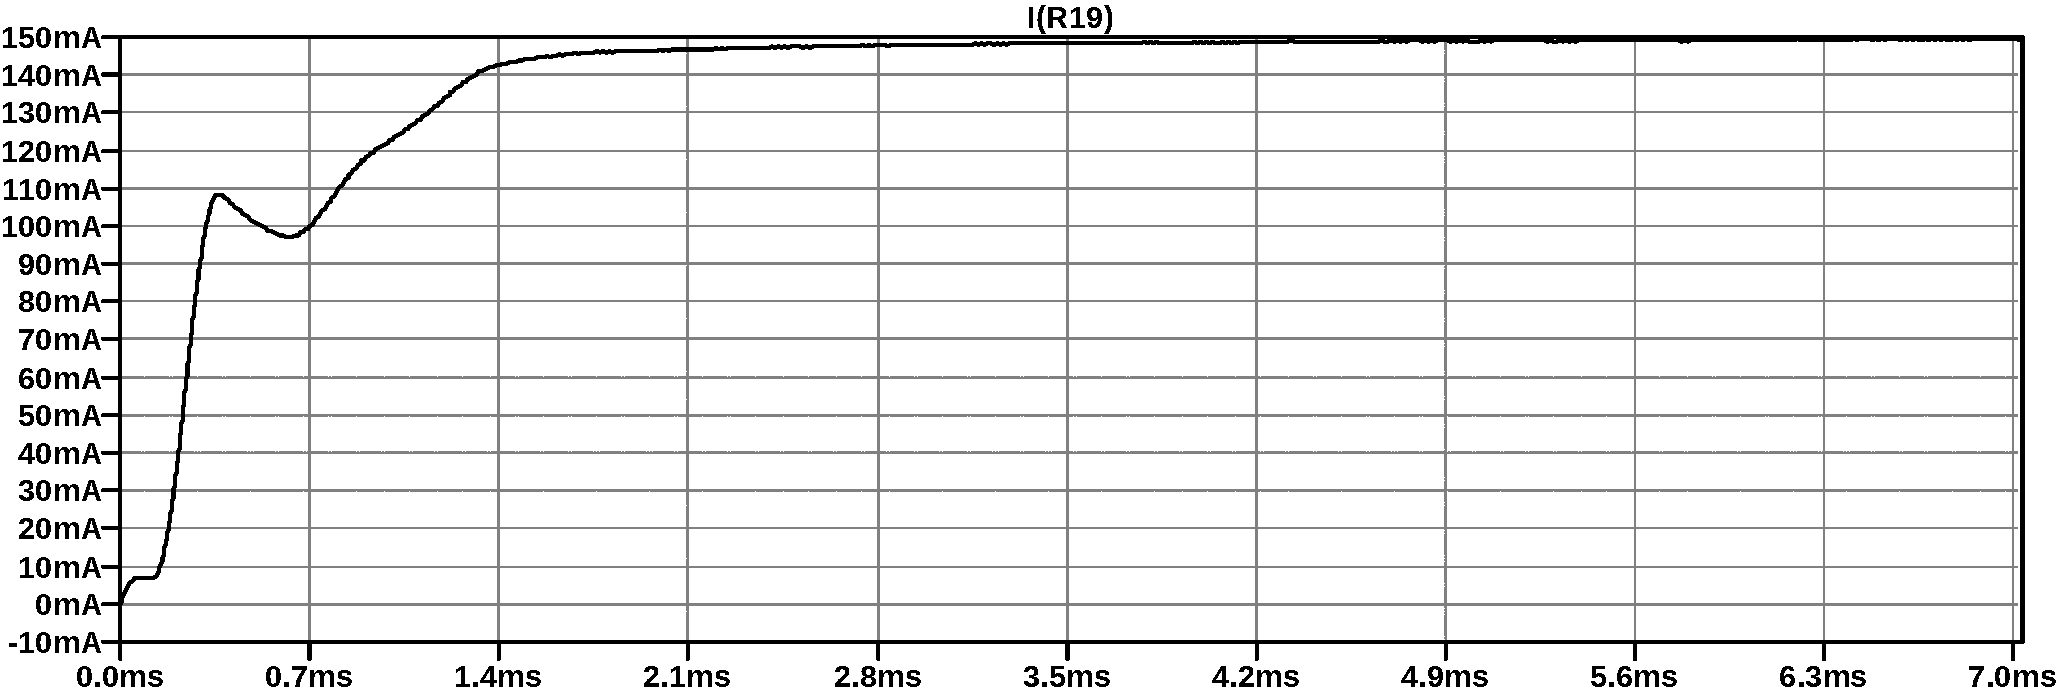
\includegraphics[width=\textwidth]{images/sim/14.pdf}
    \caption{Simulación de la corriente por la carga}
    \label{fig:sim:14}
\end{figure}

El ripple de la simulación es de 0.2mA pico a pico, mientras que el prototipo da al rededor de 5mA pico a pico máximo.

Análogamente, en las figuras \ref{fig:osc:58} y \ref{fig:sim:21ripple} se muestra el ripple de tensión en la salida salida y su simulación. En la figura \ref{fig:sim:21} se muestra la simulación de la tensión de salida durante el encendido.
% 9) Tensión de salida junto con su ripple 

\begin{figure}[H]
    \centering
    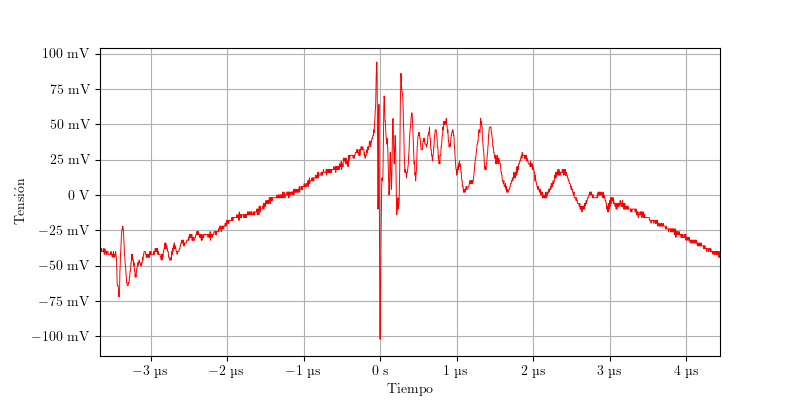
\includegraphics[width=0.8\textwidth]{images/capturas-osciloscopio/17-11-2022/58.png}
    \caption{Ripple de tensión en la carga}
    \label{fig:osc:58}
\end{figure}

\begin{figure}[H]
    \centering
    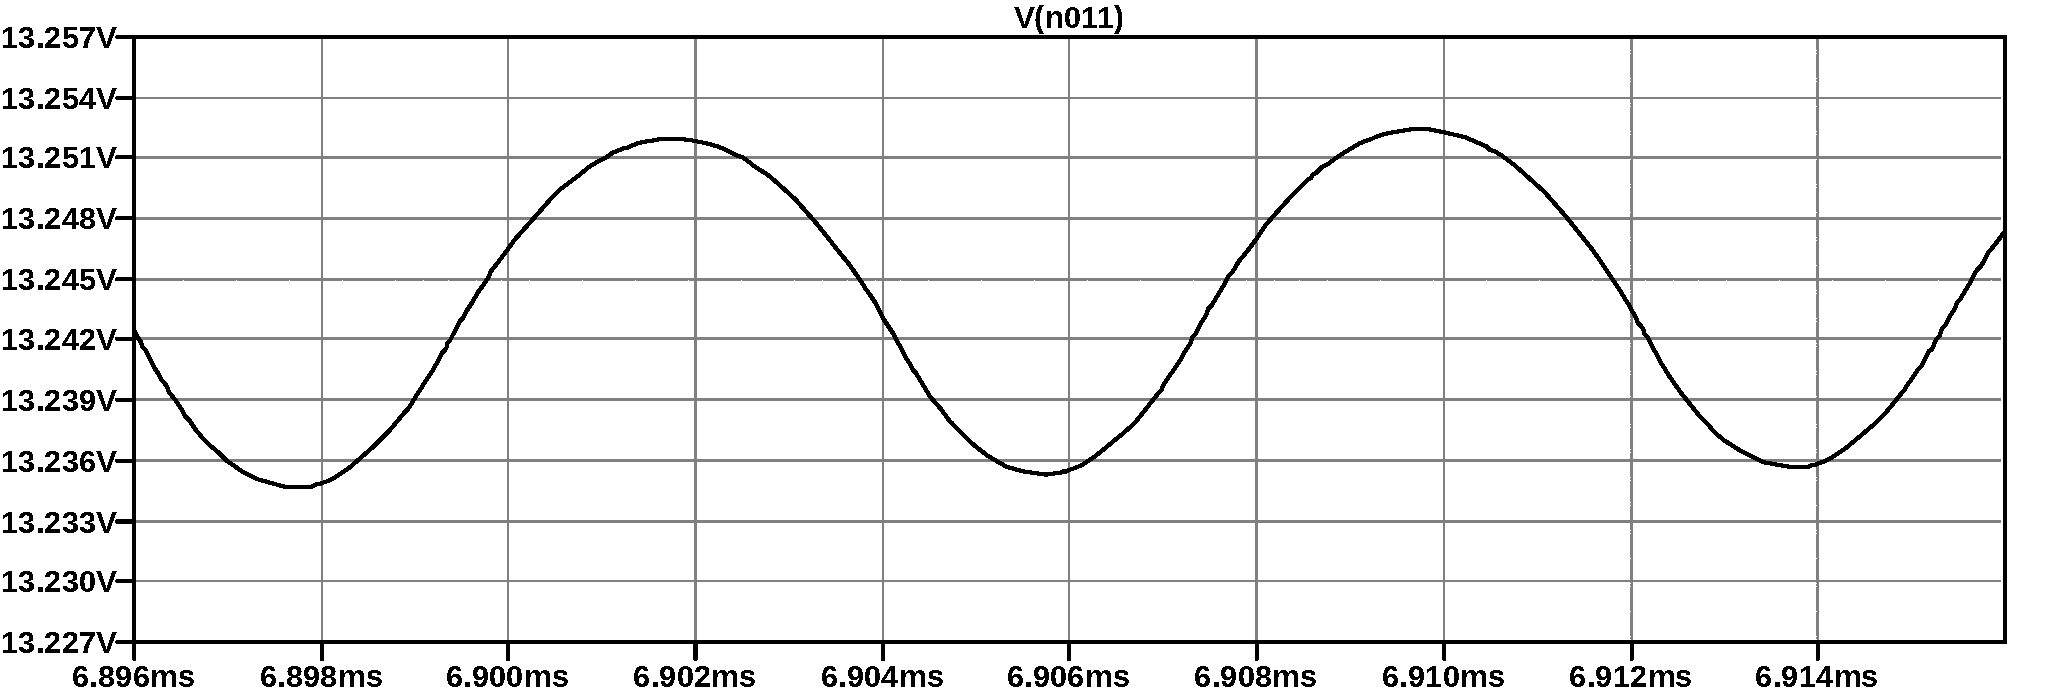
\includegraphics[width=\textwidth]{images/sim/21-ripple.pdf}
    \caption{Simulación del ripple de tensión en la carga}
    \label{fig:sim:21ripple}
\end{figure}

\begin{figure}[H]
    \centering
    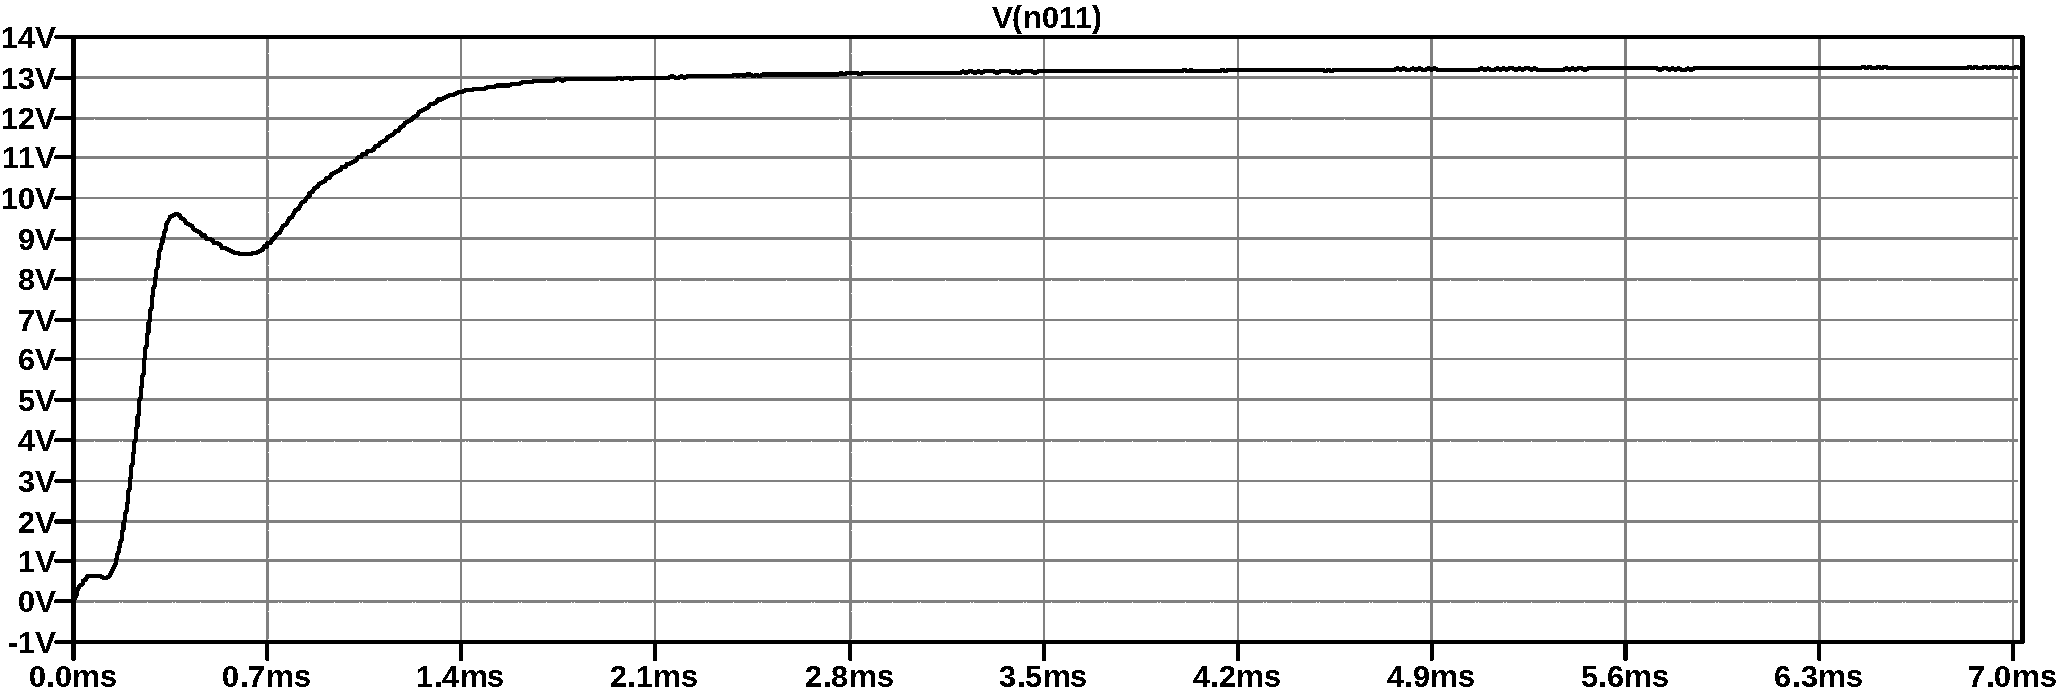
\includegraphics[width=\textwidth]{images/sim/21.pdf}
    \caption{Simulación de la tensión en la carga}
    \label{fig:sim:21}
\end{figure}

La mayor diferencia del prototipo implementado respecto a las simulaciones se obtuvo en la tensión de salida. 
Se varió la resistencia de carga conectada al convertidor y se midieron la tensión y corriente de entrada y de salida para calcular la eficiencia del circuito.
Para todas las mediciones realizadas la tensión de entrada fue de $36V$.

\begin{table}[H]
    \centering
    \begin{tabular}{lllllll}
        \hline
        \multicolumn{1}{c}{$R[\Omega]$} & \multicolumn{1}{c}{$I_i[A]$} & \multicolumn{1}{c}{$V_o[V]$} & \multicolumn{1}{c}{$I_o[A]$} & \multicolumn{1}{c}{$P_i[W]$} & \multicolumn{1}{c}{$P_o[W]$} & \multicolumn{1}{c}{$\eta[\%]$} \\ \hline
        12.6                            & 0.23                         & 5.77                         & 0.47                         & 8.28                         & 2.71                         & 32.7                           \\
        18                              & 0.23                         & 7                            & 0.4                          & 8.28                         & 2.8                          & 33.8                           \\
        24.3                            & 0.23                         & 8.3                          & 0.35                         & 8.28                         & 2.91                         & 35.1                           \\
        30.6                            & 0.23                         & 9.13                         & 0.3                          & 8.28                         & 2.74                         & 33.1                           \\
        40                              & 0.2                          & 10.2                         & 0.25                         & 7.2                          & 2.7                          & 37.5                           \\
        58                              & 0.18                         & 11.6                         & 0.2                          & 6.48                         & 2.32                         & 35.8                           \\
        80.7                            & 0.16                         & 12.4                         & 0.15                         & 5.76                         & 1.86                         & 32.3                           \\
        88.5                            & 0.16                         & 12.6                         & 0.14                         & 5.76                         & 1.76                         & 30.6                           \\ \hline
    \end{tabular}
    \caption{Resultados de las mediciones realizadas en el prototipo}
    \label{tab:mediciones}
\end{table}

% ANÁLISIS MEDICIONES

En base a la tabla \ref{tab:mediciones} se evidencia como, con ciclo de trabajo y tensión de alimentación fija, la tensión de salida varía con la carga conectada y, en consecuencia, la tensión de salida deseada de $V_{o}=12.6V$ sólo se logra para una resistencia de $R=88.5\Omega$.

% COMPARACIÓN MEDICIONES VS SIMULACIONES

En comparación con las simulaciones, como se observa en la tabla \ref{tab:mediciones_sim}, la variación de carga modifica levemente la tensión de salida pero el cambio no es tan amplio.
Por otra parte, si bien la fuente regulable de $36V$ tiene una corriente máxima de $1A$, nunca entregó la corriente esperada por simulación. 
Además, presenta una corriente de salida y una eficiencia mucho mayor en las resistencias de carga más bajas. 

\begin{table}[H]
    \centering
    \begin{tabular}{lllllll}
    \hline
    $R[\Omega]$ & $I_i[A]$ & $V_o[V]$ & $I_o[A]$ & \multicolumn{1}{c}{$P_i[W]$} & \multicolumn{1}{c}{$P_o[W]$} & \multicolumn{1}{c}{$\eta[\%]$} \\ \hline
    12.6        & 1.46     & 12.49    & 0.99     & 17.65                        & 12.39                        & 70.19                          \\
    18          & 1.33     & 12.70    & 0.71     & 13.72                        & 8.96                         & 65.31                          \\
    24.3        & 1.24     & 12.84    & 0.51     & 10.80                        & 6.60                         & 61.11                          \\
    30.6        & 1.17     & 12.98    & 0.35     & 8.07                         & 4.56                         & 56.51                          \\
    40          & 1.16     & 13.00    & 0.33     & 7.68                         & 4.23                         & 55.08                          \\
    58          & 1.12     & 13.09    & 0.23     & 6.14                         & 2.95                         & 48.05                          \\
    80.7        & 1.10     & 13.17    & 0.16     & 5.11                         & 2.15                         & 42.07                          \\
    88.5        & 1.10     & 13.24    & 0.15     & 4.89                         & 1.95                         & 39.88                          \\ \hline
    \end{tabular}
    \caption{Resultados de las mediciones en la simulación}
    \label{tab:mediciones_sim}
\end{table}

% COMPARACIÓN VO: MARCO TEÓRICO Y SIMULACIÓN 

Si bien según lo analizado en el marco teórico la tensión de salida resulta independiente de la carga, el leve cambio en la simulación puede deberse a que, con el objetivo de simplificar el análisis del convertidor forward, se consideró el modelo ideal de todos sus componentes. 
Esto se evidencia en el simulador donde, al utilizar modelos reales de los semiconductores, la tensión de salida comienza a variar levemente con la carga.

% COMPARACIÓN VO: SIMULACIÓN Y MEDICIONES

En la figura \ref{fig:comparacion} se ilustran de manera gráfica los resultados obtenidos en la tensión de salida con la variación de la carga.

\begin{figure}[H]
    \centering
    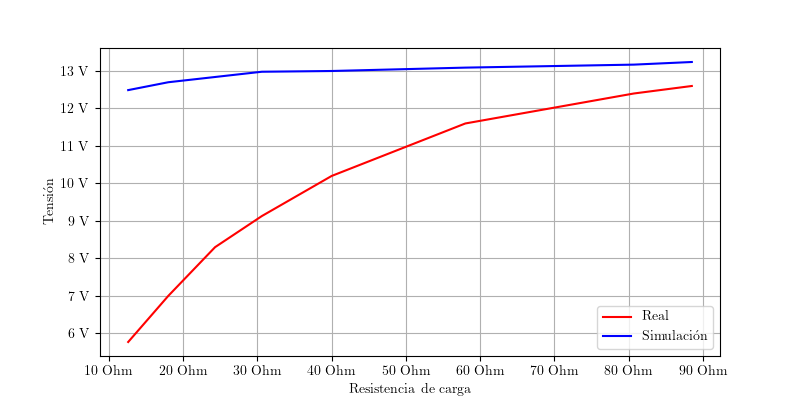
\includegraphics[width=0.8\textwidth]{images/comparacion-general.png}
    \caption{Comparación entre los resultados de las simulaciones y las mediciones realizadas}
    \label{fig:comparacion}
\end{figure}

La gran diferencia puede deberse a elementos parásitos del circuito, cuyas pérdidas aumentan con la corriente de carga y provocan caídas de tensión que no se han considerado en la simulación.
Además, si bien en la teoría analizada y en las simulaciones del prototipo los transistores conmutan de forma simultánea, en las mediciones realizadas se aprecia un retardo entre la señal de excitación del MOSFET de lado bajo y la del lado alto. 
Es decir, para la frecuencia de conmutación elegida, el transformador del driver no tiene un tiempo despreciable de encendido y apagado como se describió en la nota de aplicación \cite{gatedrivers}.  
En consecuencia, como se observa en la tabla \ref{tab:estados}, se tiene un total de 4 estados en cada ciclo de conmutación.

\begin{table}[H]
    \centering
    \begin{tabular}{ccc}
    \hline
    Estado & MOSFET de lado bajo & MOSFET de lado alto \\ \hline
    1      & OFF                 & OFF                 \\
    2      & ON                  & OFF                 \\
    3      & ON                  & ON                  \\
    4      & OFF                 & ON                  \\ \hline
    \end{tabular}
    \caption{Estados de conmutación del convertidor forward}
    \label{tab:estados}
\end{table}

Se corroboró con el simulador que la tensión a la salida del convertidor se ve afectada por los 2 estados adicionales a ambos MOSFETs encendidos y ambos MOSFETs apagados. Por lo tanto, se concluye que dichos estados indeseados y la existencia de elementos parásitos en el circuito que no fueron considerados en la simulación son las principales causas de la gran diferencia en la tensión de salida.  

En base al análisis realizado, es de entender que en la práctica los convertidores funcionan a lazo cerrado sensando la tensión y/o corriente de salida, y por medio de un sistema de realimentación ajustan el ciclo de trabajo para obtener una tensión de salida constante ante los cambios de carga o la tensión de entrada del convertidor.